\chapter{Analisys and result discussion}
In the previous section the author has explained the steps followed to forecast electricity prices and explore the different predictors' influence. We are now discussing the configuration fixed for the hourly, daily, monthly and yearly setups, and the results obtained on each case.

For each scenario has to be selected the length of the time series to be used, the forecasting horizon, the number of lags and the predictors to be included. This has been selected with the help of a topic expert, concretely my Thesis' Supervisor.

In the situations where ARIMA is used to forecast, the length of the window size is an hyperparameter that has to be tuned.

Before starting, just mentioning that before creating this section some initial experiments have been done. On them, the author noticed that Support Vector Machine models weren't performing good in any situation. Even though they can surpass other models performance, the forecasts are normally flat and similar to a Dummy Regressor, losing most of the variability. This is why if a SVM or a DR appear in the top of the table they are discarded and the following best model is taken.



\section{Hourly analysis}
In this case the author is working with a 6 months data window. It has been decided to make 168 hours ahead forecasts (1 week). The lags in use try to model the autocorrelation, and are the following: 1, 2, 12, 23, 24, 36, 71, 72, 167 and 168. Apart, other predictors are included to add extra information to the model:

\begin{itemize}
    \item \textbf{Date predictors:} Hour, day and day of week.
    \item \textbf{Demand:} The total energy demand.
    \item \textbf{Generation:} Wind, hydropower, nuclear, solar, combined cycle and coal generation technologies measurements.
\end{itemize}

Cross validation is applied using 20 windows, with step size of 25.

As the author mentioned, the energy market should have changed due to the Covid pandemic and specially to the war in Ukraine. This differences between current and past market will be analyzed.

\subsection{Pre-pandemic scenario}
The data used for the pre-pandemic scenario experiments goes from 2018-10-01 to 2019-03-31, before the increase in energy prices shown in Figure \ref{fig:spot-price-series-month}. In Table \ref{tab:cv-hourly-prep} you can find the performance of different models for the cross validation phase. The best one is a Random Forest, it is the one the author will use to make the final forecast.

\begin{table}[H]
\centering
\begin{tabular}{@{}l|l|l@{}}
\toprule
Model & MASE     & Fit time     \\ \midrule
RF    & 2.76181  & 1940.086432  \\
GBT   & 2.938516 & 14009.034606 \\
kNN   & 3.939263 & 17.24593     \\
SVR   & 4.252531 & 5547.920132  \\
DR    & 4.741289 & 4.483376     \\ \bottomrule
\end{tabular}
\caption{Model performance comparison trained over the hourly pre-pandemic energy price.}
\label{tab:cv-hourly-prep}
\end{table}

The final forecast is done as explained in Chapter \ref{ch:methodology}, using the train split to build the model and the test to give a final evaluation of the performance. The results are shown in Figure \ref{fig:forecast-hourly-pre}, obtaining a MASE=2.23.

\begin{figure}[H]
\centering
    \caption{Final forecasting of hourly pre-pandemic energy price.}
    \label{fig:forecast-hourly-pre}
    \fbox{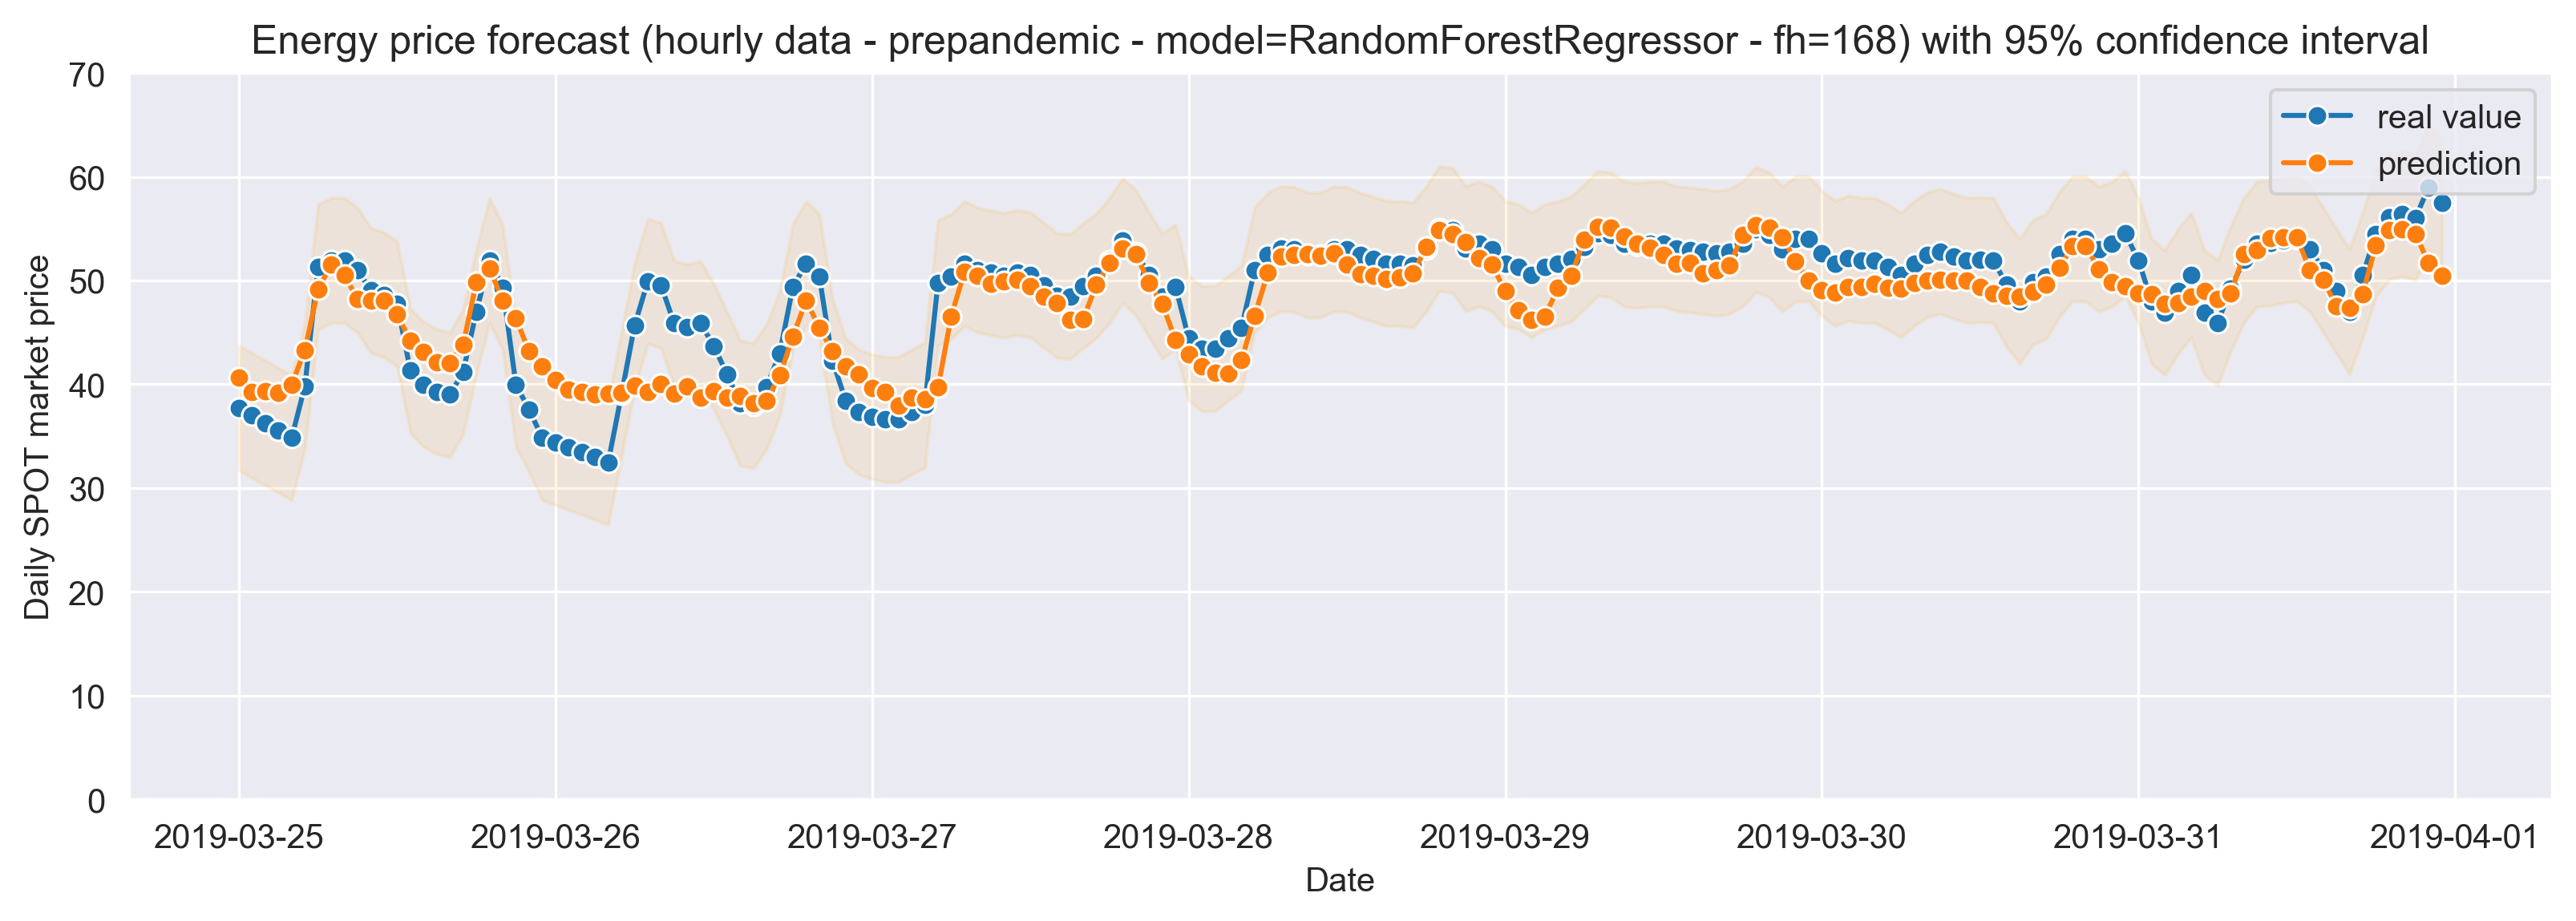
\includegraphics[scale=0.4]{images/analysis/forecast-hourly-pre}}
\end{figure}

Which are the predictors that are specially influencing this forecast? In Figure \ref{fig:shap-hourly-pre} you can see them, both for fh=1 and fh=168.

In the first case, the first lag has a lot of importance, high SHAP values are found for many test points. Concretely, if the lag takes a low value (blue color), the response value will tend to be low too. Lag two has also some importance, but in this case a low value in the lag means a higher value in the response. Combined cycle generation and hour seem to have some importance, but not very high.

In the second case, the forecast is not so dependent of the first lag, as the response (fh=168) is further away from it. Combined cycle, coal and hydropower generation are the most influential in the price.

\begin{figure}[H]
\centering
    \begin{subfigure}{.45\textwidth}
        \centering
        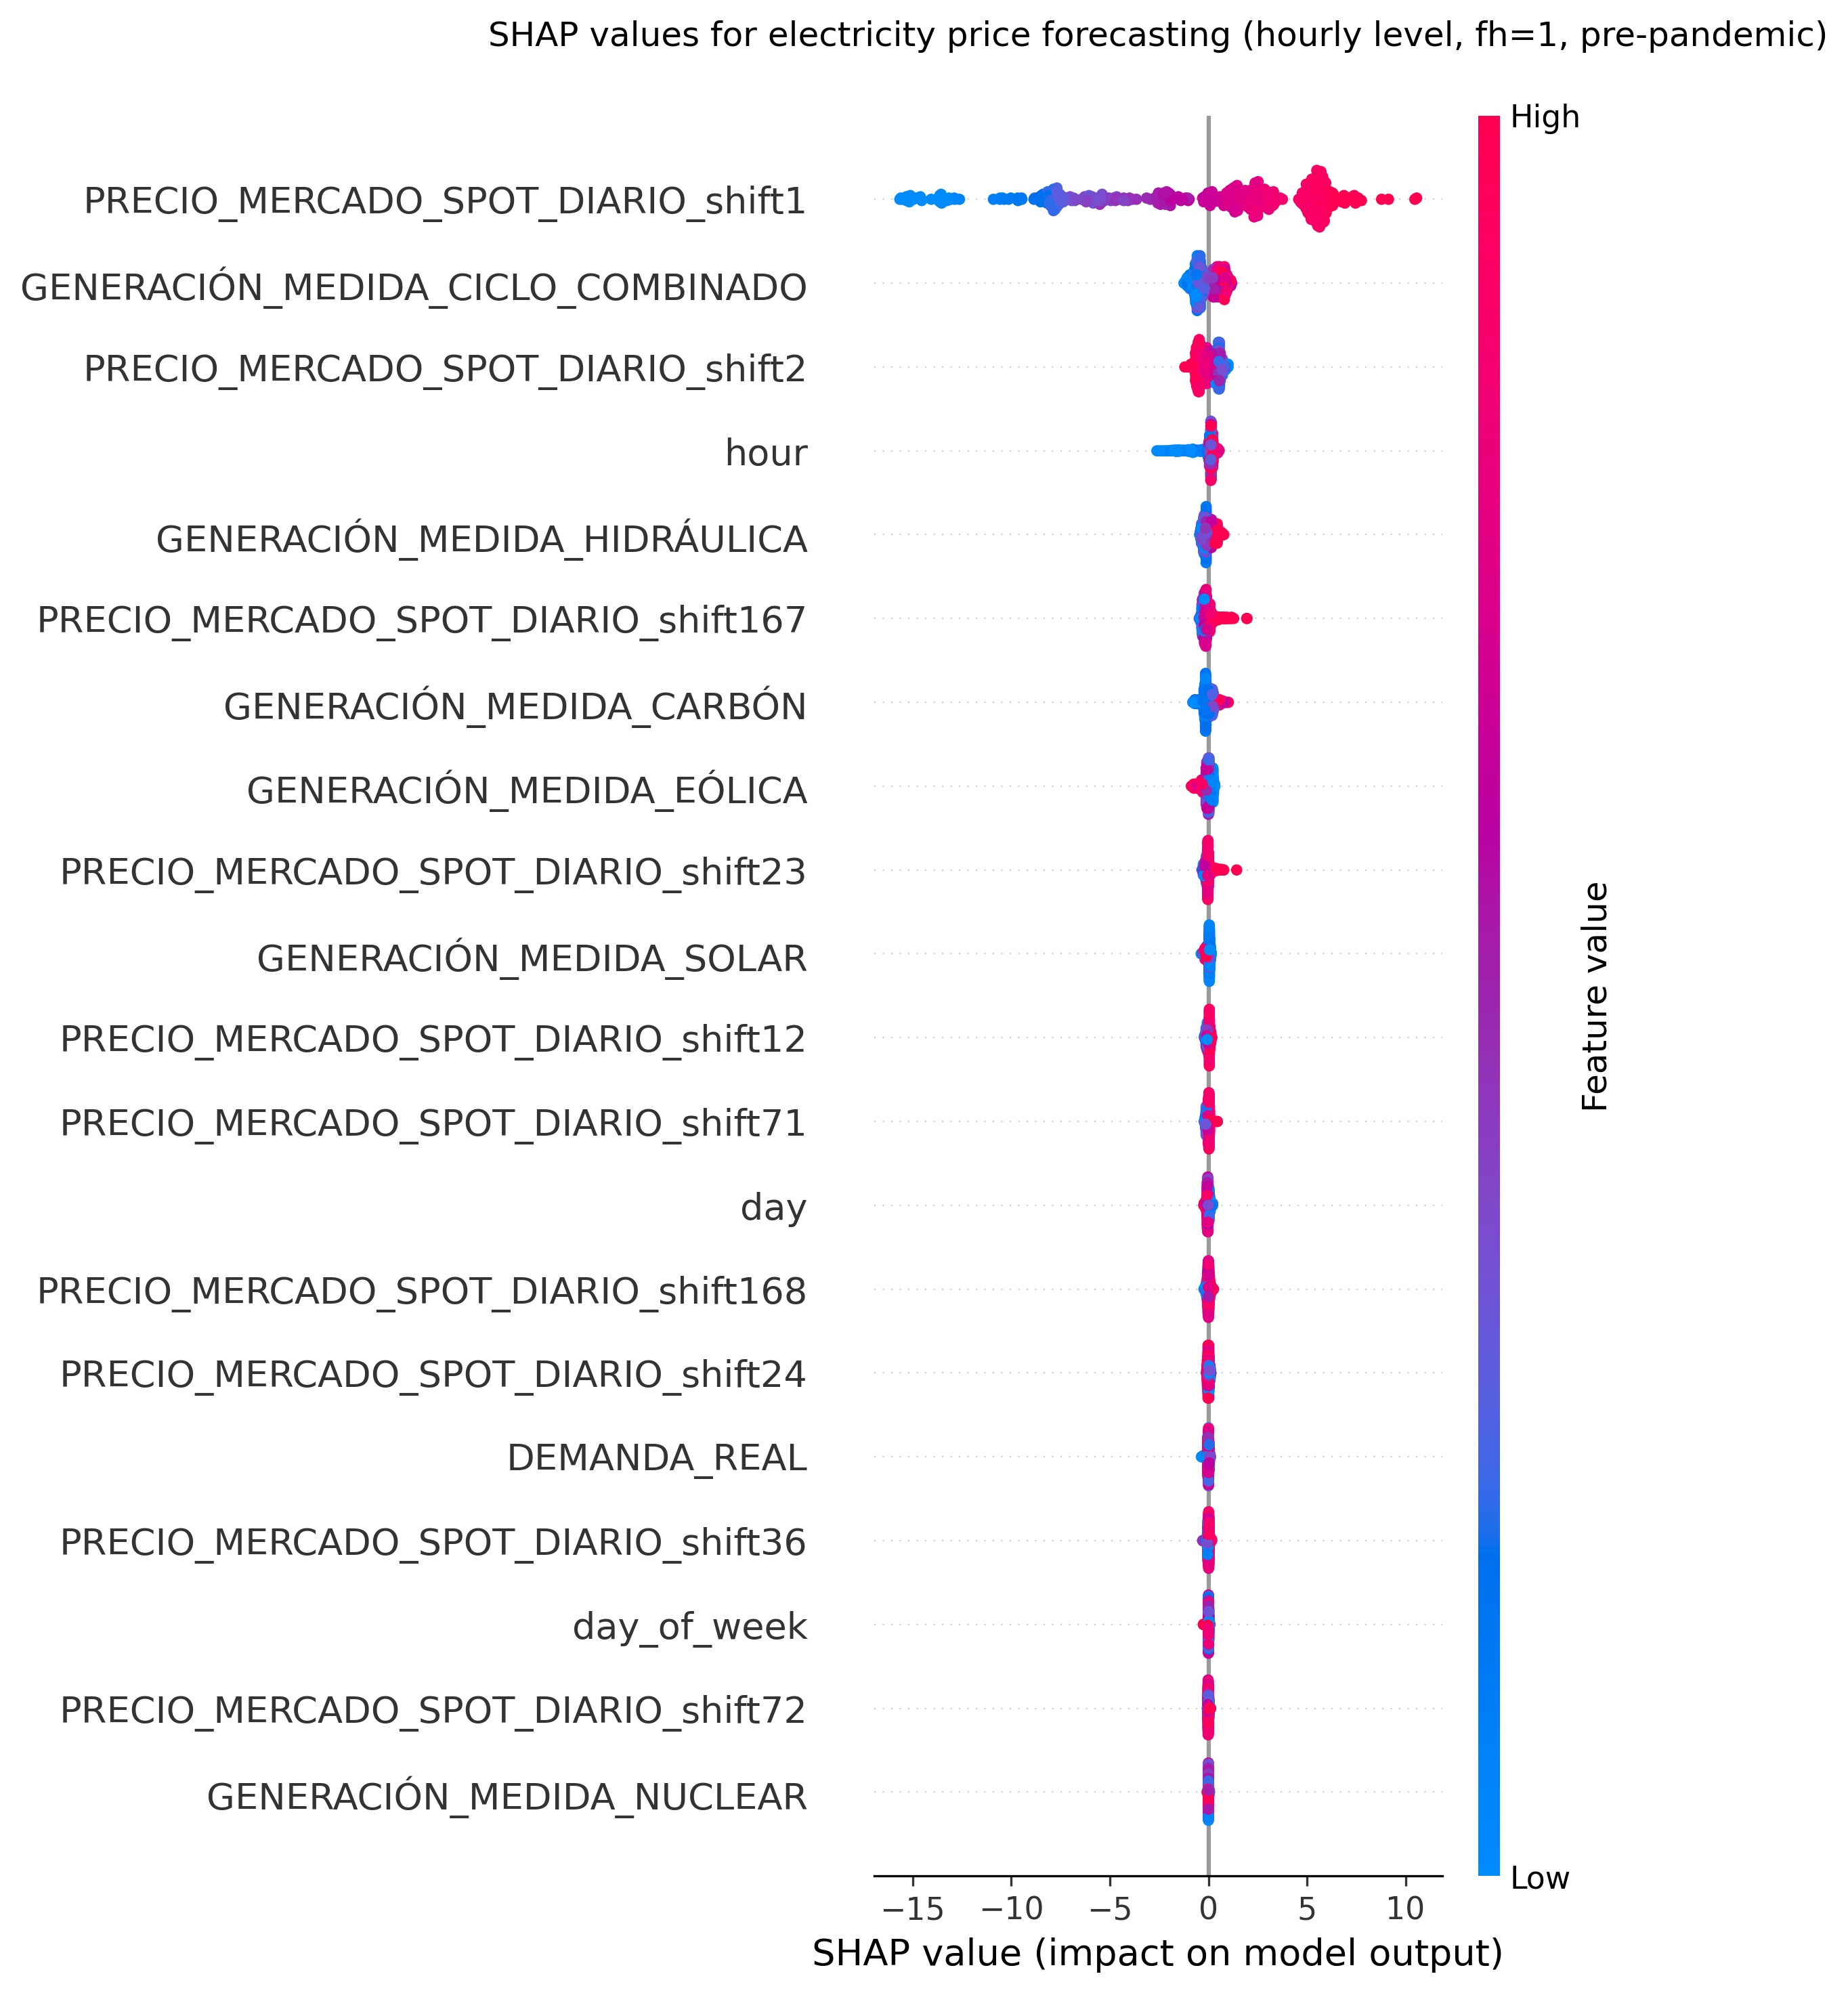
\includegraphics[width=1\linewidth]{images/analysis/shap-hourly-pre-1}
        \caption{fh=1}
    \end{subfigure}
    \begin{subfigure}{.45\textwidth}
        \centering
        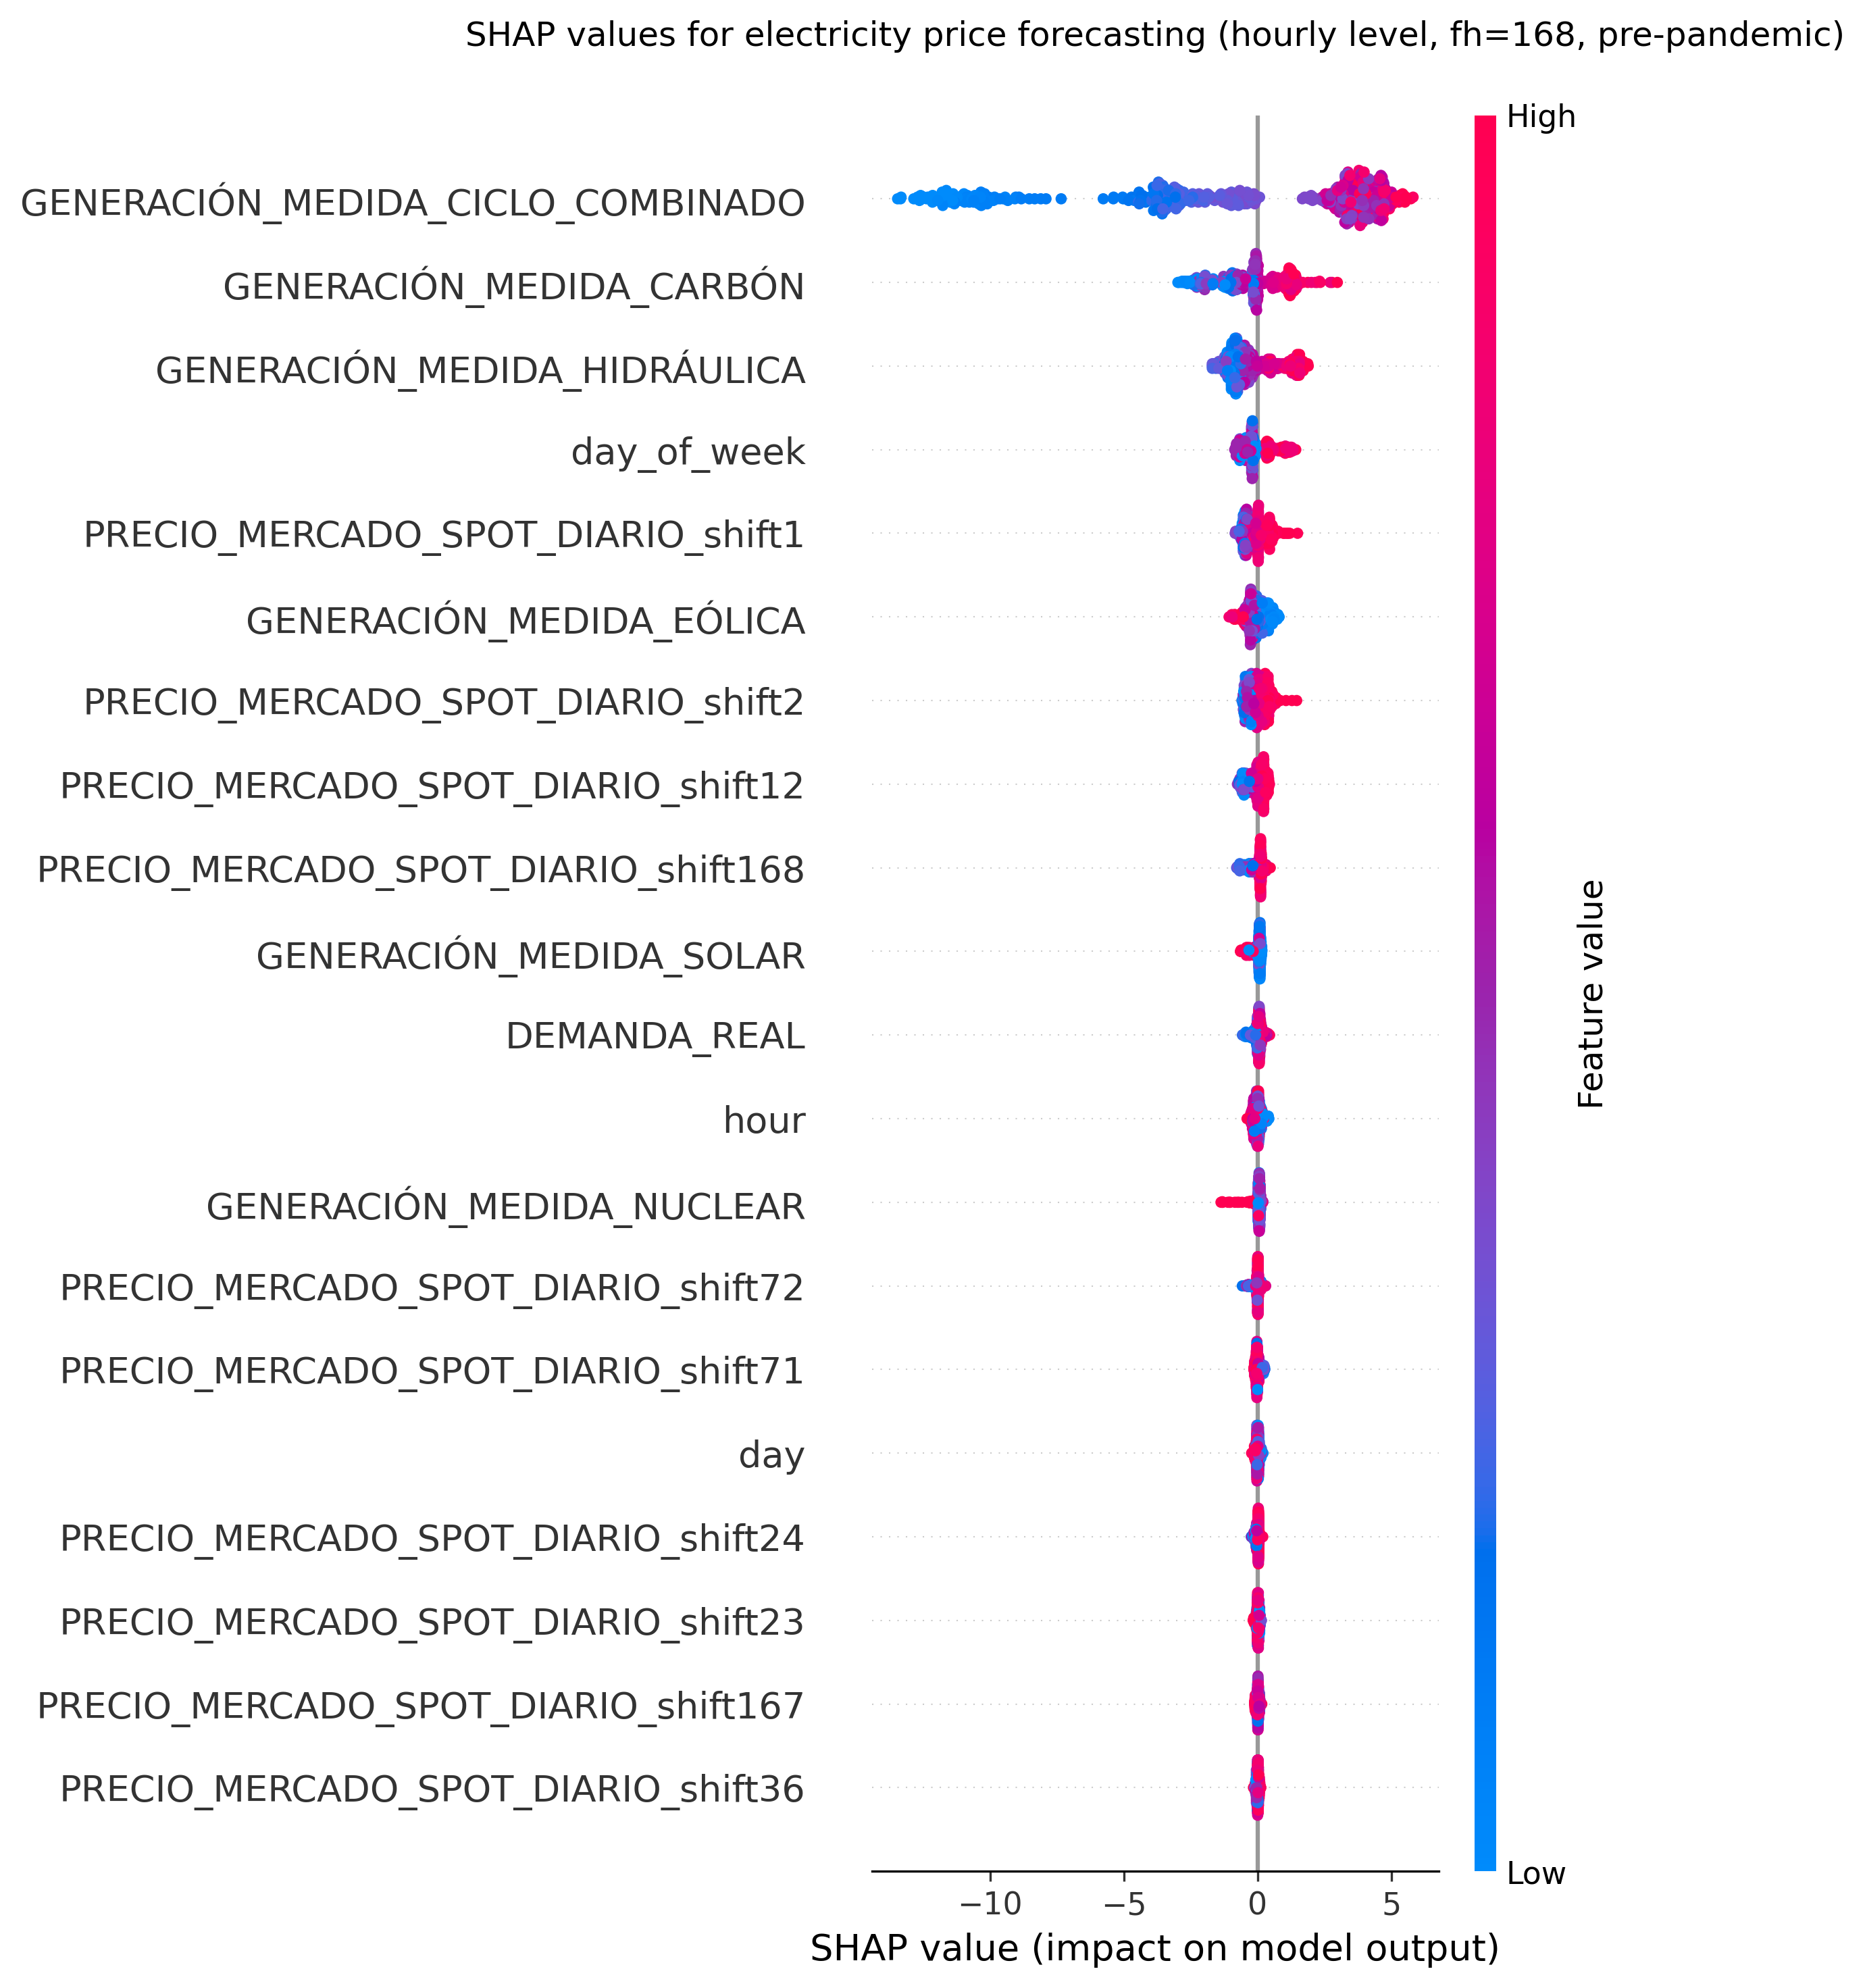
\includegraphics[width=1\linewidth]{images/analysis/shap-hourly-pre-168}
        \caption{fh=168}
    \end{subfigure}

    \caption{SHAP values for the hourly pre-pandemic energy price forecasting.}
    \label{fig:shap-hourly-pre}
\end{figure}

\subsection{Post-Unkraine war scenario}
The data in use goes from 2022-10-01 to 2023-03-31. In the model selection stage the author obtains the results described in Table \ref{tab:cv-hourly-post}.

% Please add the following required packages to your document preamble:
% \usepackage{booktabs}
\begin{table}[H]
\centering
\begin{tabular}{@{}l|l|l@{}}
\toprule
Model & MASE     & Fit time     \\ \midrule
GBT   & 3.713739 & 5196.343993  \\
RF    & 3.755286 & 13717.128606 \\
SVM   & 3.901001 & 2823.434254  \\
kNN   & 3.932622 & 3.564837     \\
DR    & 4.770888 & 7.018414     \\ \bottomrule
\end{tabular}
\caption{Model performance comparison trained over the hourly post-Ukraine war energy prices.}
\label{tab:cv-hourly-post}
\end{table}

The best-performing model, in this post-war scenario, is the one based on Gradient Boosted Trees (GBT). The final forecast is shown in Figure \ref{fig:forecast-hourly-post} with a MASE of 4.01.

\begin{figure}[H]
\centering
    \caption{Final forecasting of hourly post-war energy price.}
    \label{fig:forecast-hourly-post}
    \fbox{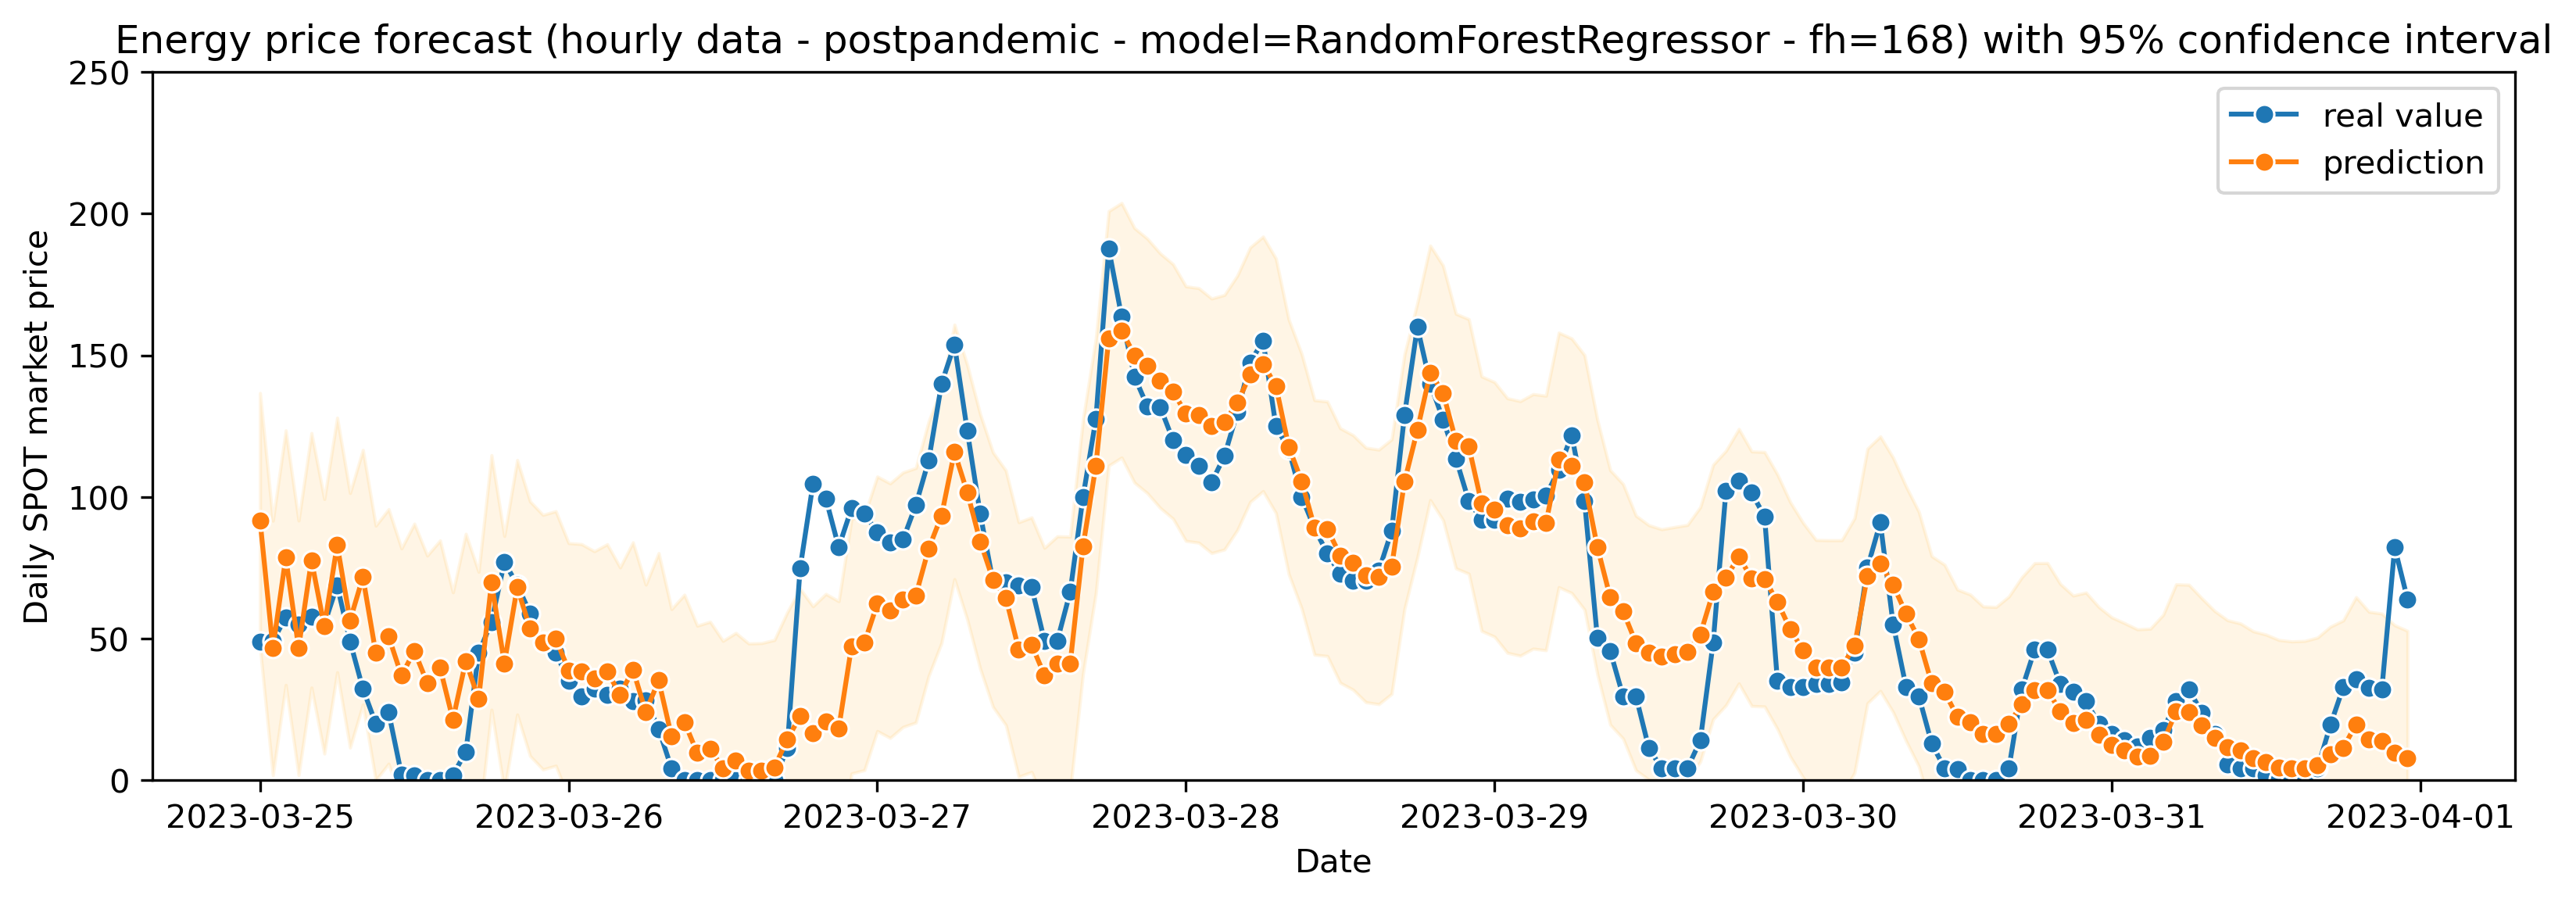
\includegraphics[scale=0.4]{images/analysis/forecast-hourly-post}}
\end{figure}

In this case, the most important predictors are shown in Figure \ref{fig:shap-hourly-post}. Compared with the pre-pandemic series, we find similar predictors for fh=1, but with higher weight for combined cycle generation. For fh=168, combined cycle generation is also increasing its repercussion in prices. This makes sense, as gas prices have increased a lot and the electricity price series have done it too.

\begin{figure}[H]
\centering
    \begin{subfigure}{.45\textwidth}
        \centering
        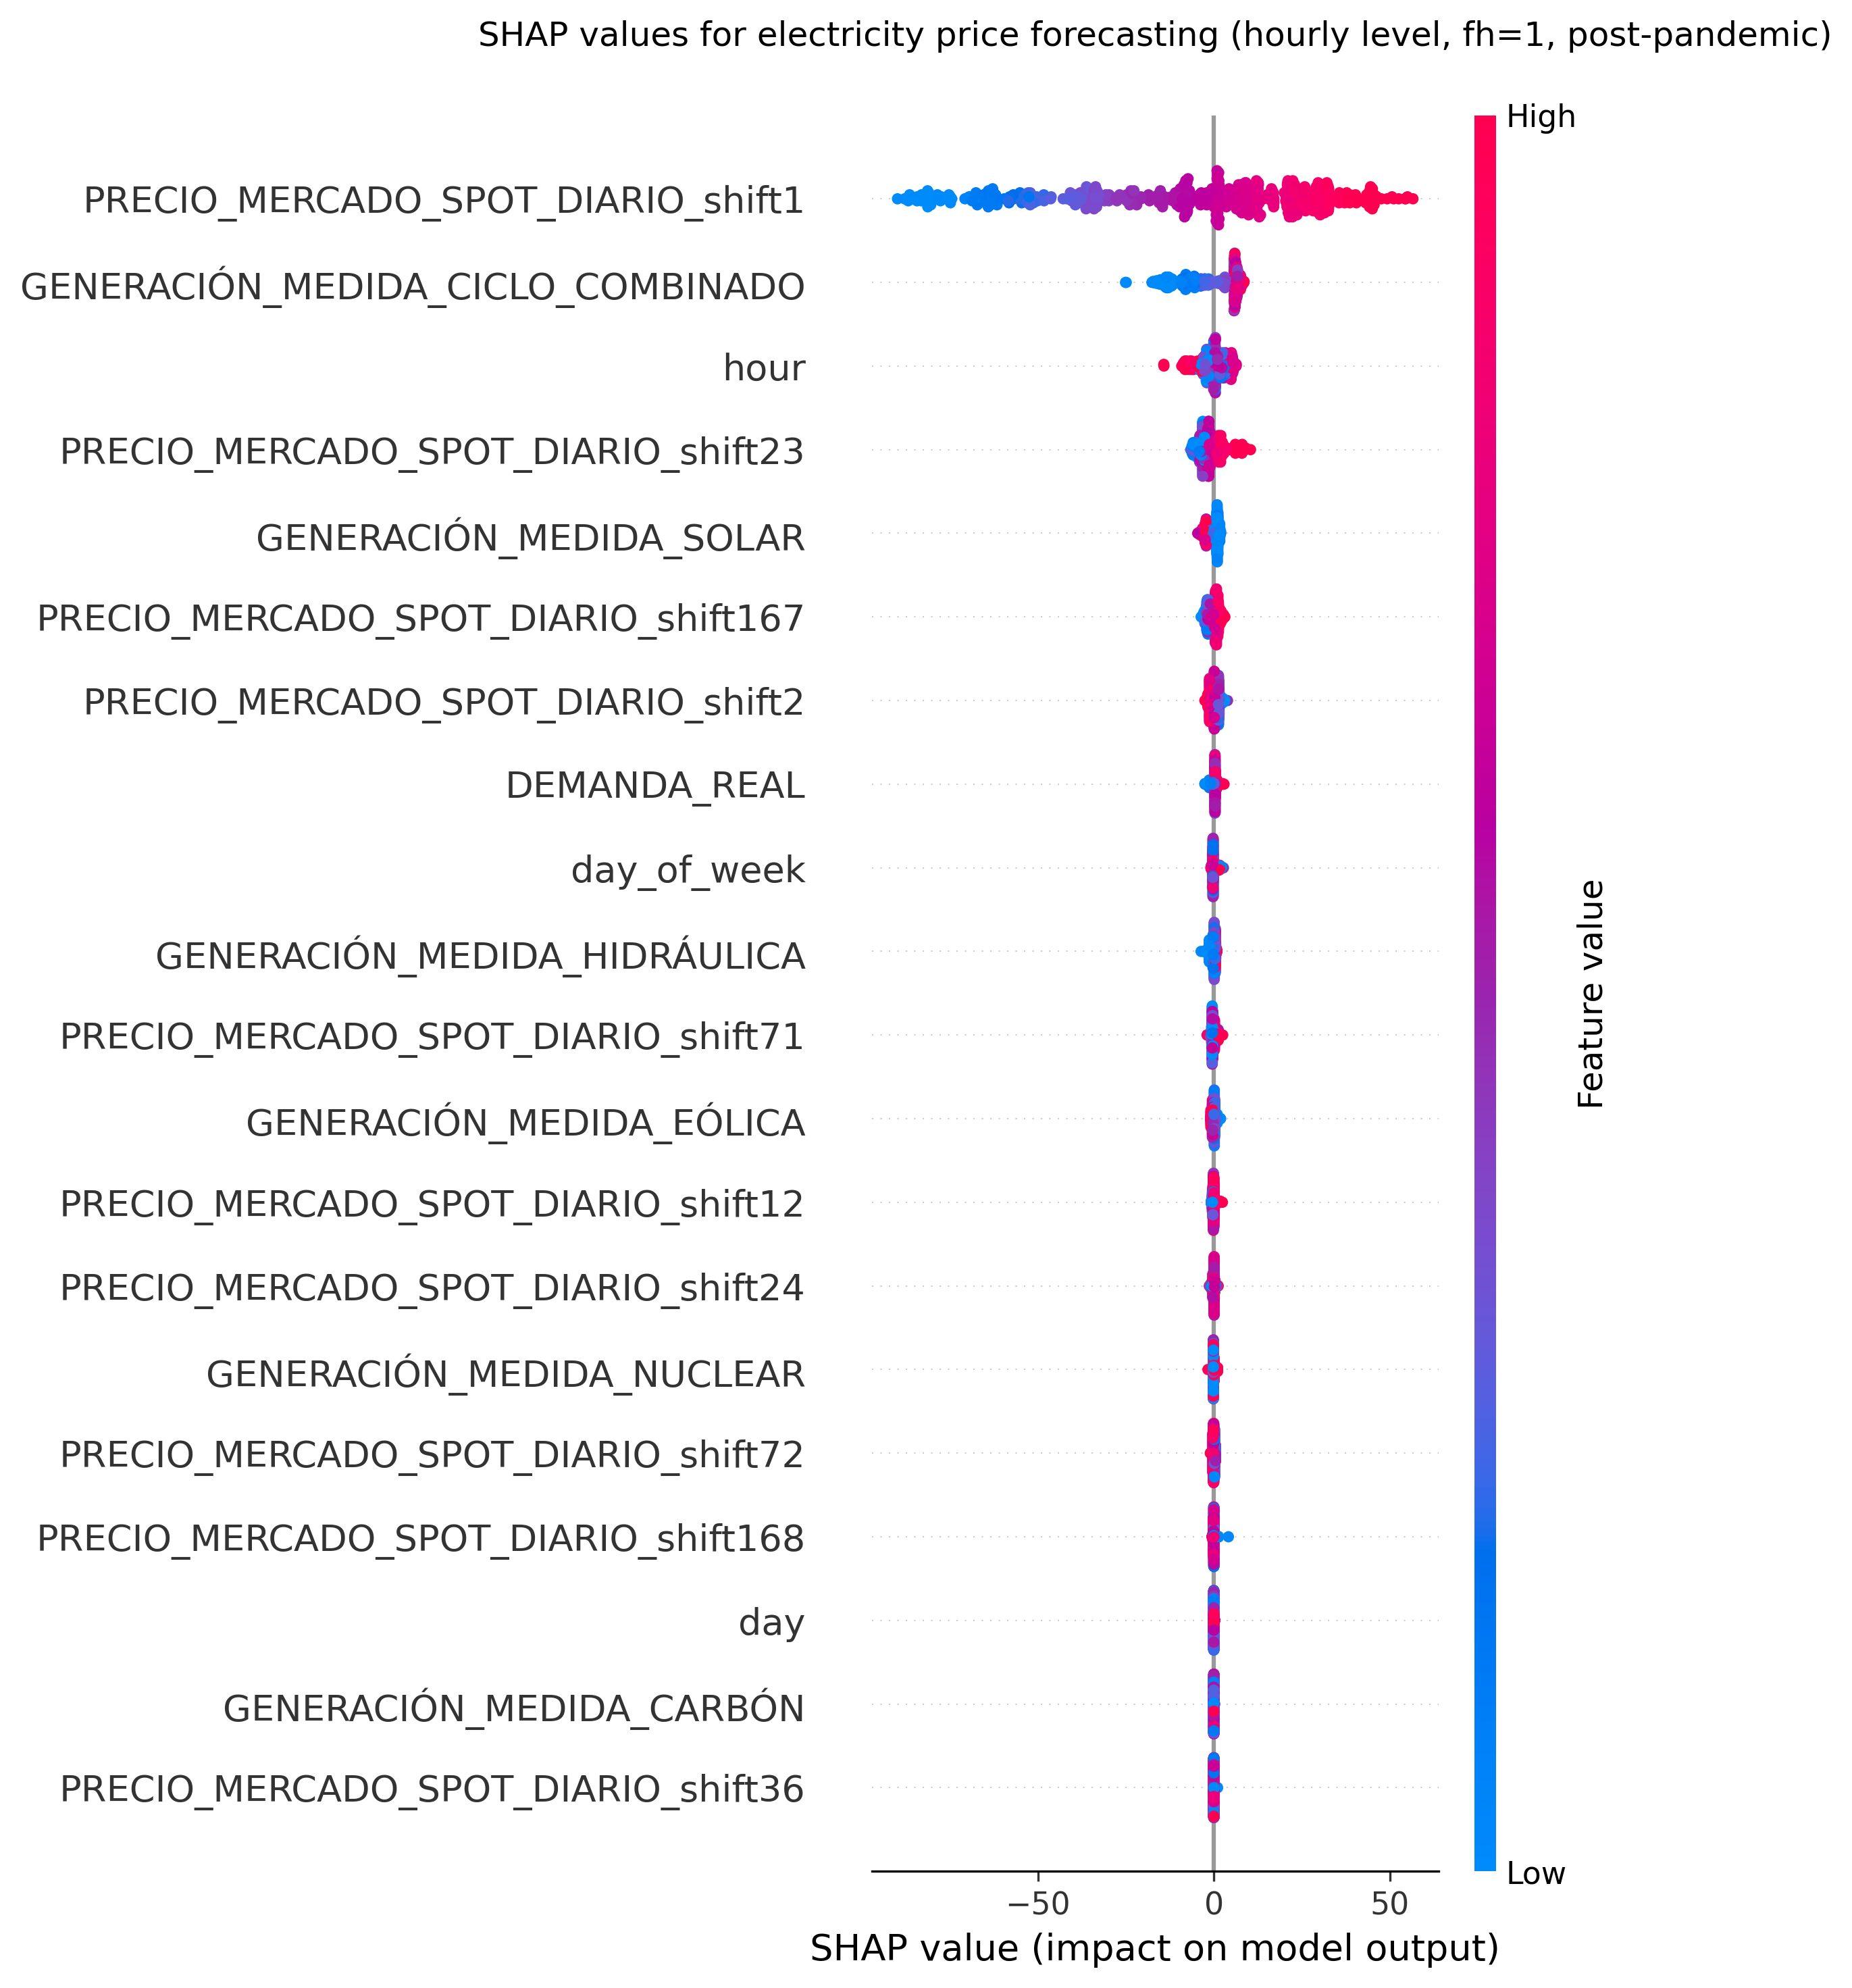
\includegraphics[width=1\linewidth]{images/analysis/shap-hourly-post-1}
        \caption{fh=1}
    \end{subfigure}
    \begin{subfigure}{.45\textwidth}
        \centering
        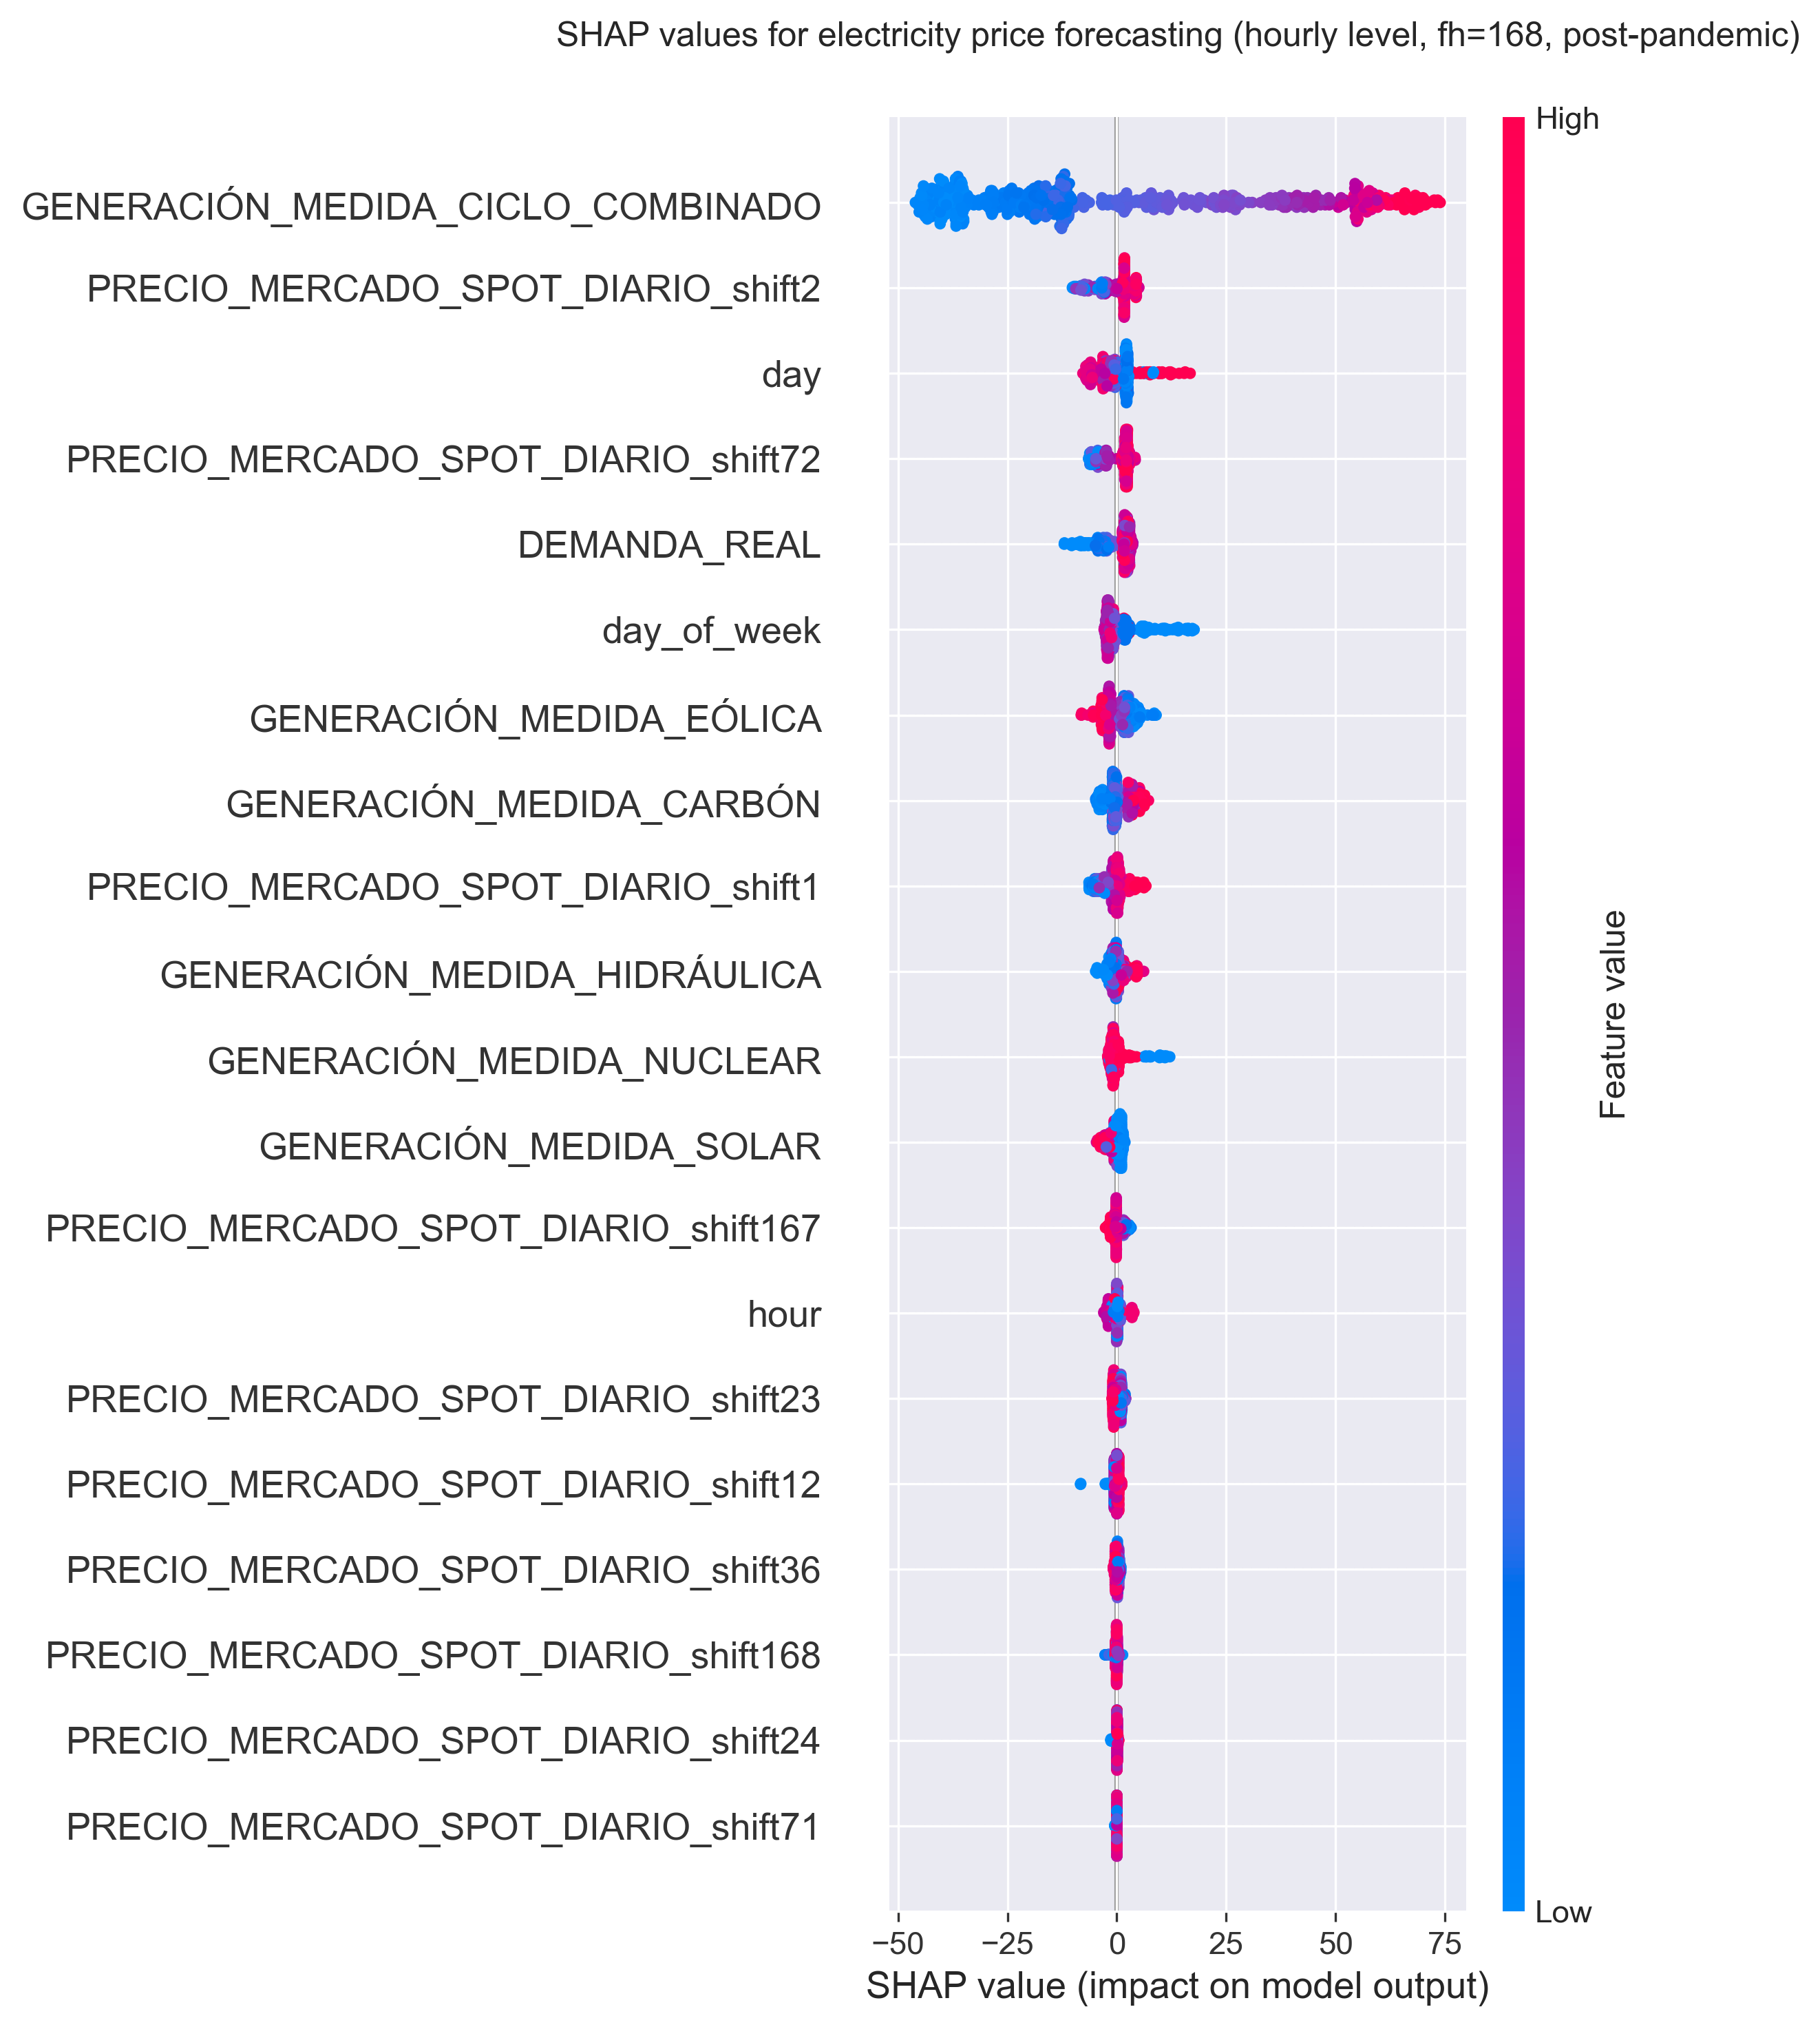
\includegraphics[width=1\linewidth]{images/analysis/shap-hourly-post-168}
        \caption{fh=168}
    \end{subfigure}

    \caption{SHAP values for the hourly post-war energy price forecasting.}
    \label{fig:shap-hourly-post}
\end{figure}


\subsection{Result discussion}
The models that have performed the best are those related with tree ensembles, both RF and GBT. With them, reasonably good forecasts have been obtained, getting a low MASE score. Finally, the main difference in the influence of predictors before and after Covid crisis and the war in Ukraine is that now the gas price is affecting more the electricity price than before.





\section{Daily analysis}
For the daily aggregation data from 2 years is used, producing 30 days ahead forecasts. The lags added as predictors are 2, 6, 7, 13, 14, 28, 30 and 31, apart we use demand and generation as before and some new predictors:

\begin{itemize}
    \item \textbf{Date predictors:} Day, day of week, week of the year and month.
    \item \textbf{Demand:} The total energy demand.
    \item \textbf{Generation:} Wind, hydropower, nuclear, solar, combined cycle and coal generation technologies measurements.
    \item \textbf{Gas price}
    \item \textbf{Coal price}
    \item \textbf{EU $CO_2$ allowances price}
\end{itemize}

\noindent Cross validation is applied again using 20 windows, but in this case the step size is 1.

\subsection{Pre-pandemic scenario}
The data used for the pre-pandemic scenario experiments goes from 2018-04-01 to 2020-03-31. The model which performed the best was based on Gradient Boosting Trees (GBT), obtaining 2.215 as MASE.

\begin{table}[H]
\centering
\begin{tabular}{l|l|l}
\hline
Model & MASE     & Fit time   \\ \hline
GBT   & 2.215121 & 181.750649 \\
RF    & 2.748981 & 404.297131 \\
kNN   & 2.796314 & 0.885529   \\
SVM   & 4.444936 & 12.376585  \\
DR    & 4.452648 & 0.43246    \\ \hline
\end{tabular}
\caption{Model performance comparison trained over the daily pre-pandemic energy price.}
\label{tab:cv-daily-prep}
\end{table}

Nevertheless, as has been explained in Chapter \ref{ch:methodology}, for the medium and long term forecasts ARIMA models are also tested.

\begin{table}[H]
\centering
\begin{tabular}{@{}l|l|l@{}}
\toprule
Model          & MASE     & Fit time   \\ \midrule
AutoARIMA\_400 & 0.929604 & 197.504757 \\
AutoARIMA\_300 & 1.117683 & 78.747226  \\
AutoARIMA\_200 & 1.248828 & 97.493102  \\
AutoARIMA\_500 & 1.88596  & 114.225986 \\ \bottomrule
\end{tabular}
\caption{ARIMA performance comparison trained over the hourly pre-pandemic energy price.}
\label{tab:arima-daily-prep}
\end{table}

And they are working very good, specially the one using a 400 points window for training.

\begin{figure}[H]
\centering
    \caption{Final forecasting of daily pre-pandemic energy price.}
    \label{fig:forecast-arima-daily-pre}
    \fbox{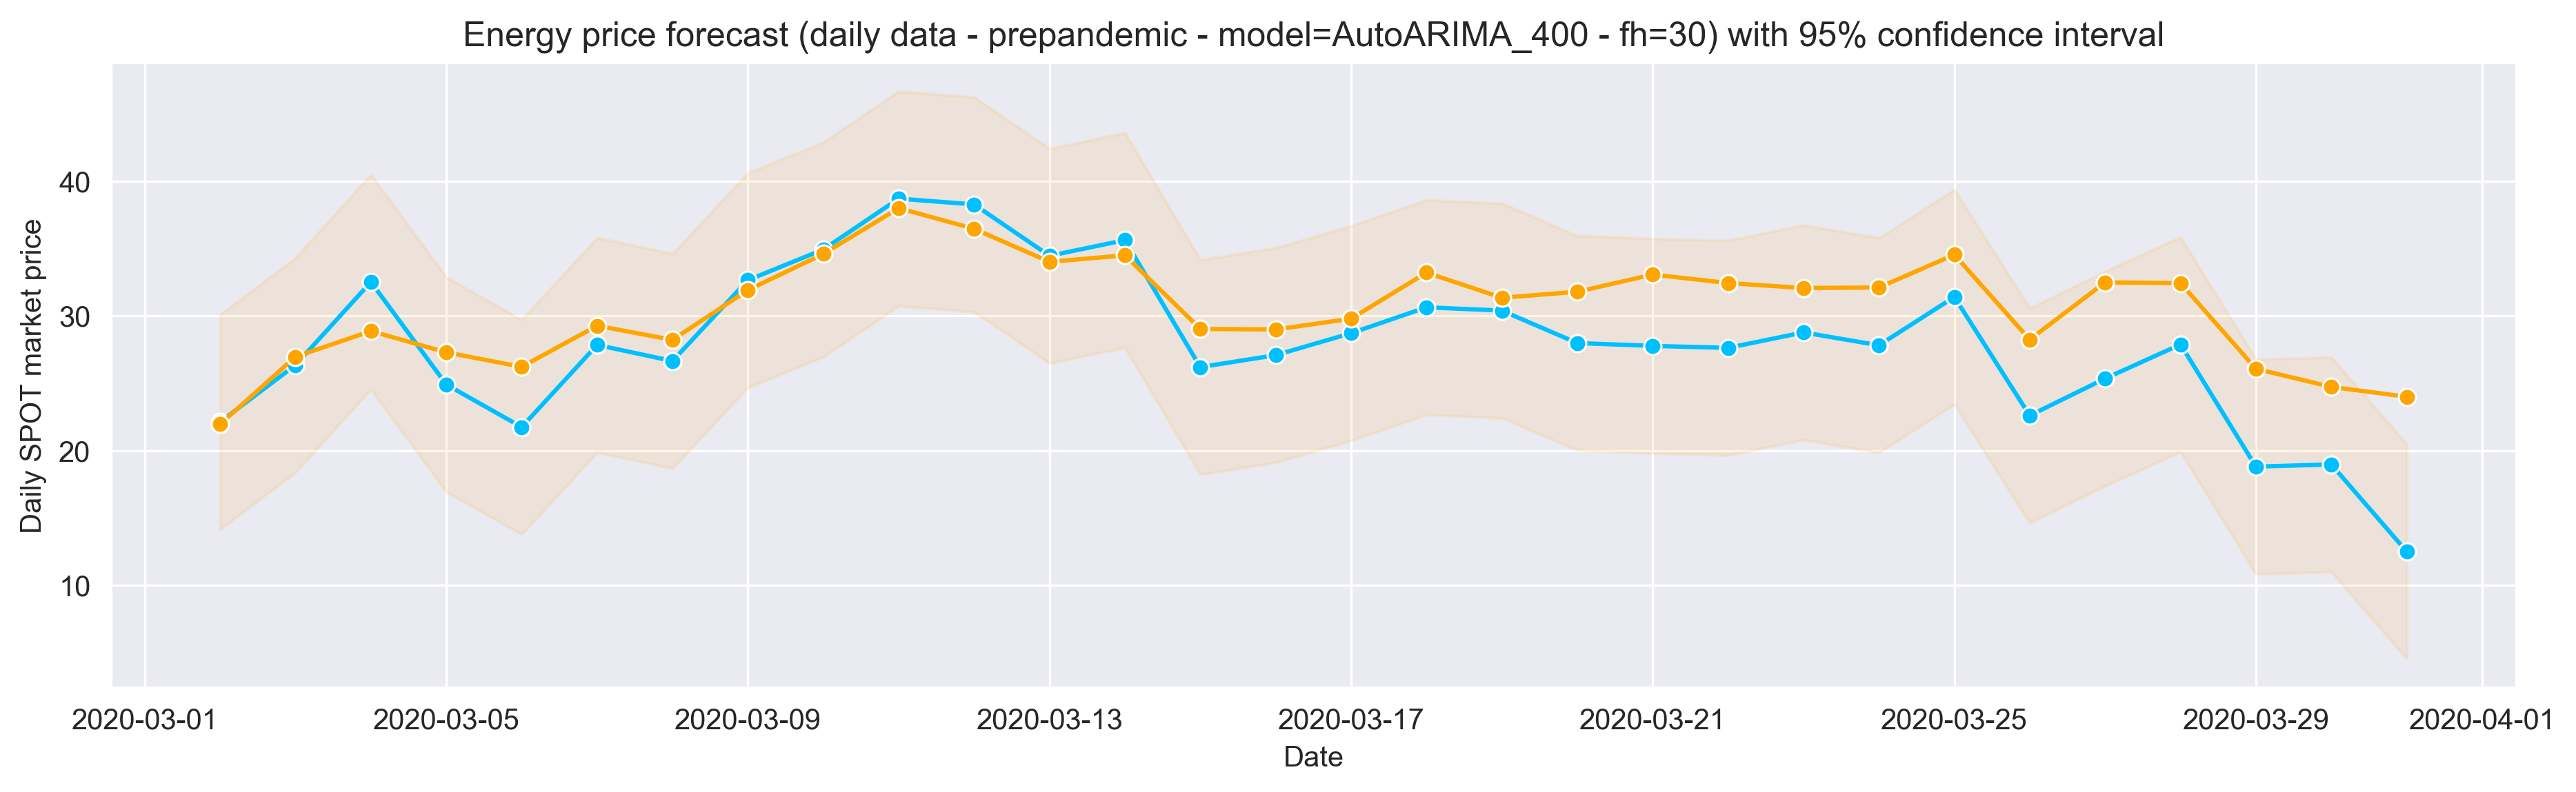
\includegraphics[scale=0.4]{images/analysis/forecast-arima-daily-pre}}
\end{figure}

Even though ARIMA is the best performing model, SHAP values are computed over GBT. As it has been explained in Chapter \ref{ch:methodology} the SHAP package is not directly compatible with ARIMA.

\begin{figure}[H]
\centering
    \begin{subfigure}{.45\textwidth}
        \centering
        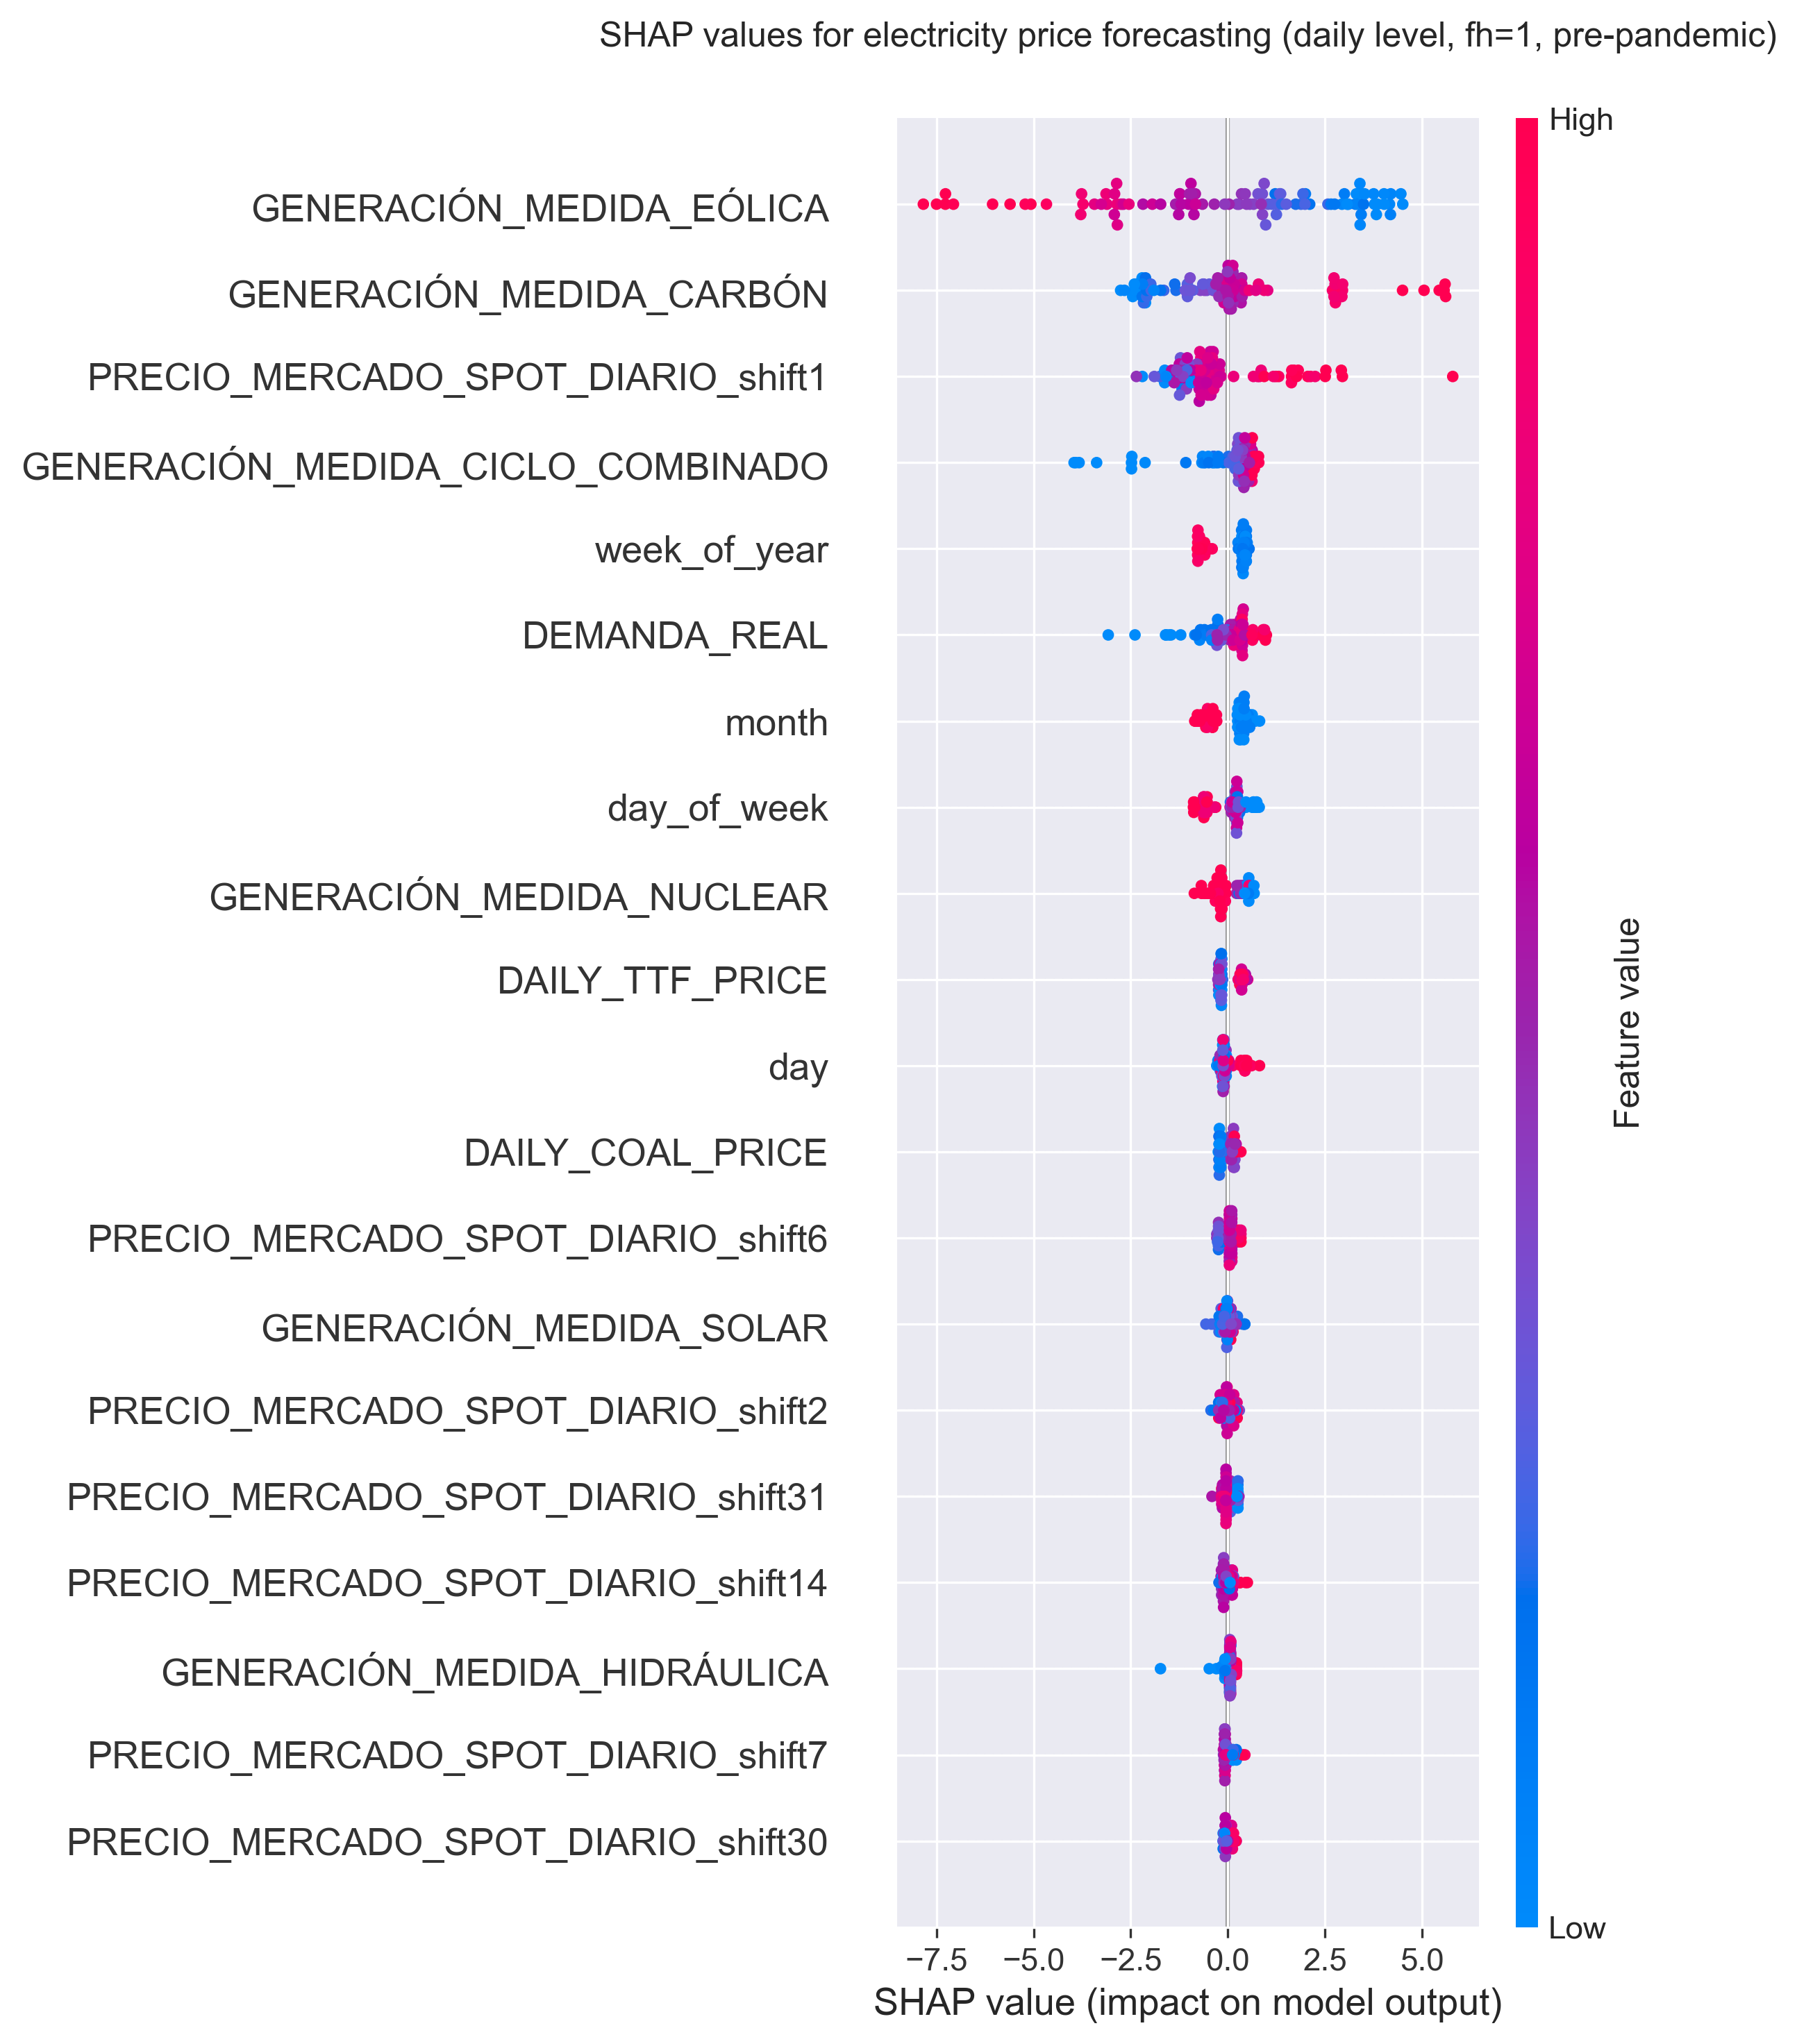
\includegraphics[width=1\linewidth]{images/analysis/shap-daily-pre-1}
        \caption{fh=1}
    \end{subfigure}
    \begin{subfigure}{.45\textwidth}
        \centering
        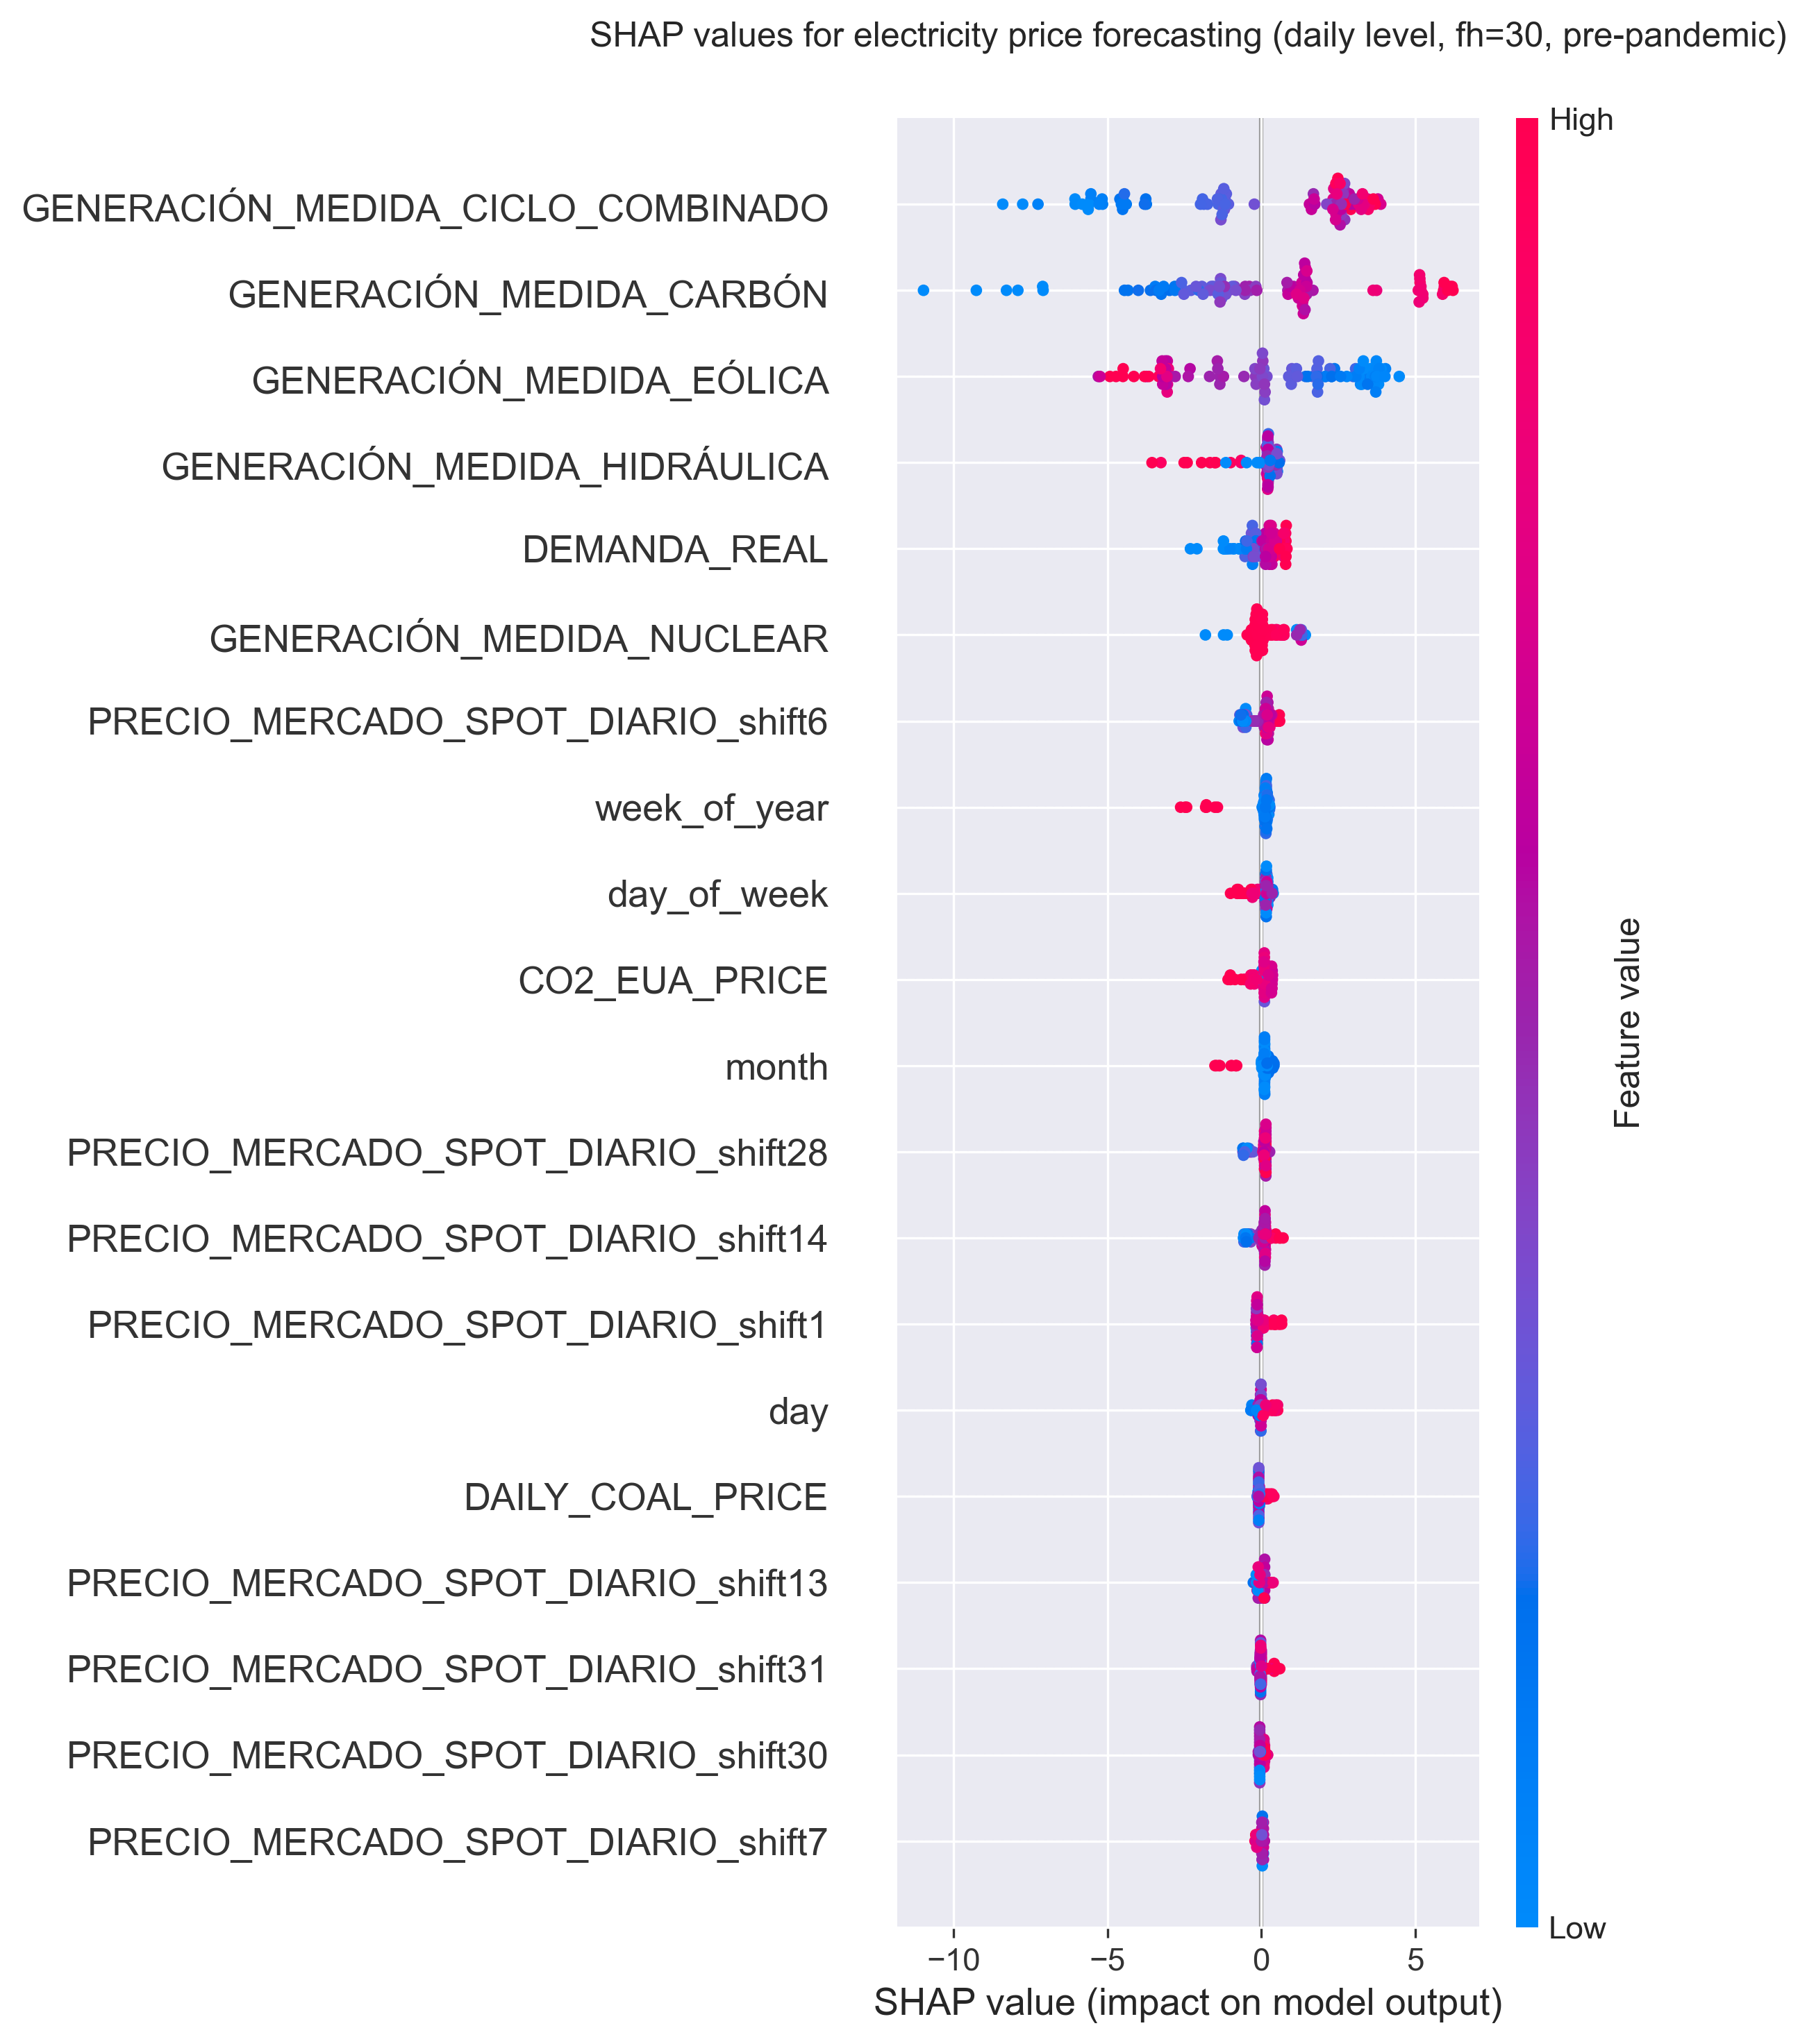
\includegraphics[width=1\linewidth]{images/analysis/shap-daily-pre-30}
        \caption{fh=30}
    \end{subfigure}

    \caption{SHAP values for the daily pre-pandemic energy price forecasting.}
    \label{fig:shap-daily-pre}
\end{figure}

The results show that when predicting fh=1, the use of wind generation reduces the cost of electricity. The inverse happens for coal and combined cycle. Apart, the first lag is influencing the forecast.

When predicting fh=168 something similar happens, but this lag is now much less informative.

\subsection{After-Unkraine war scenario}
Let's now explore the after-war scenario. Data in use goes from 2021-04-01 to 2023-03-31, and the best performing model is also GBT.

\begin{table}[H]
\centering
\begin{tabular}{l|l|l}
\hline
Model & MASE     & Fit time    \\ \hline
GBT   & 4.897767 & 696.383714  \\
DR    & 4.907985 & 0.430406    \\
RF    & 5.892628 & 1388.050782 \\
SVM   & 6.872439 & 144.108247  \\
kNN   & 7.408178 & 0.93499     \\ \hline
\end{tabular}
\caption{Model performance comparison trained over the daily post-war energy price.}
\label{tab:cv-daily-post}
\end{table}

Again, ARIMA is improving the results of ML based models so it will be used to make the final forecasts.

\begin{table}[H]
\centering
\begin{tabular}{@{}l|l|l@{}}
\toprule
Model          & MASE     & Fit time   \\ \midrule
AutoARIMA\_500 & 1.695899 & 87.581615  \\
AutoARIMA\_300 & 2.162655 & 147.963091 \\
AutoARIMA\_400 & 2.548488 & 129.669448 \\
AutoARIMA\_200 & 2.698293 & 97.405607  \\ \bottomrule
\end{tabular}
\caption{ARIMA performance comparison trained over the daily post-war energy price.}
\label{tab:arima-daily-post}
\end{table}

Concretely, the best performing ARIMA uses a window of size 500.

\begin{figure}[H]
\centering
    \caption{Final forecasting of daily post-war energy price.}
    \label{fig:forecast-arima-daily-post}
    \fbox{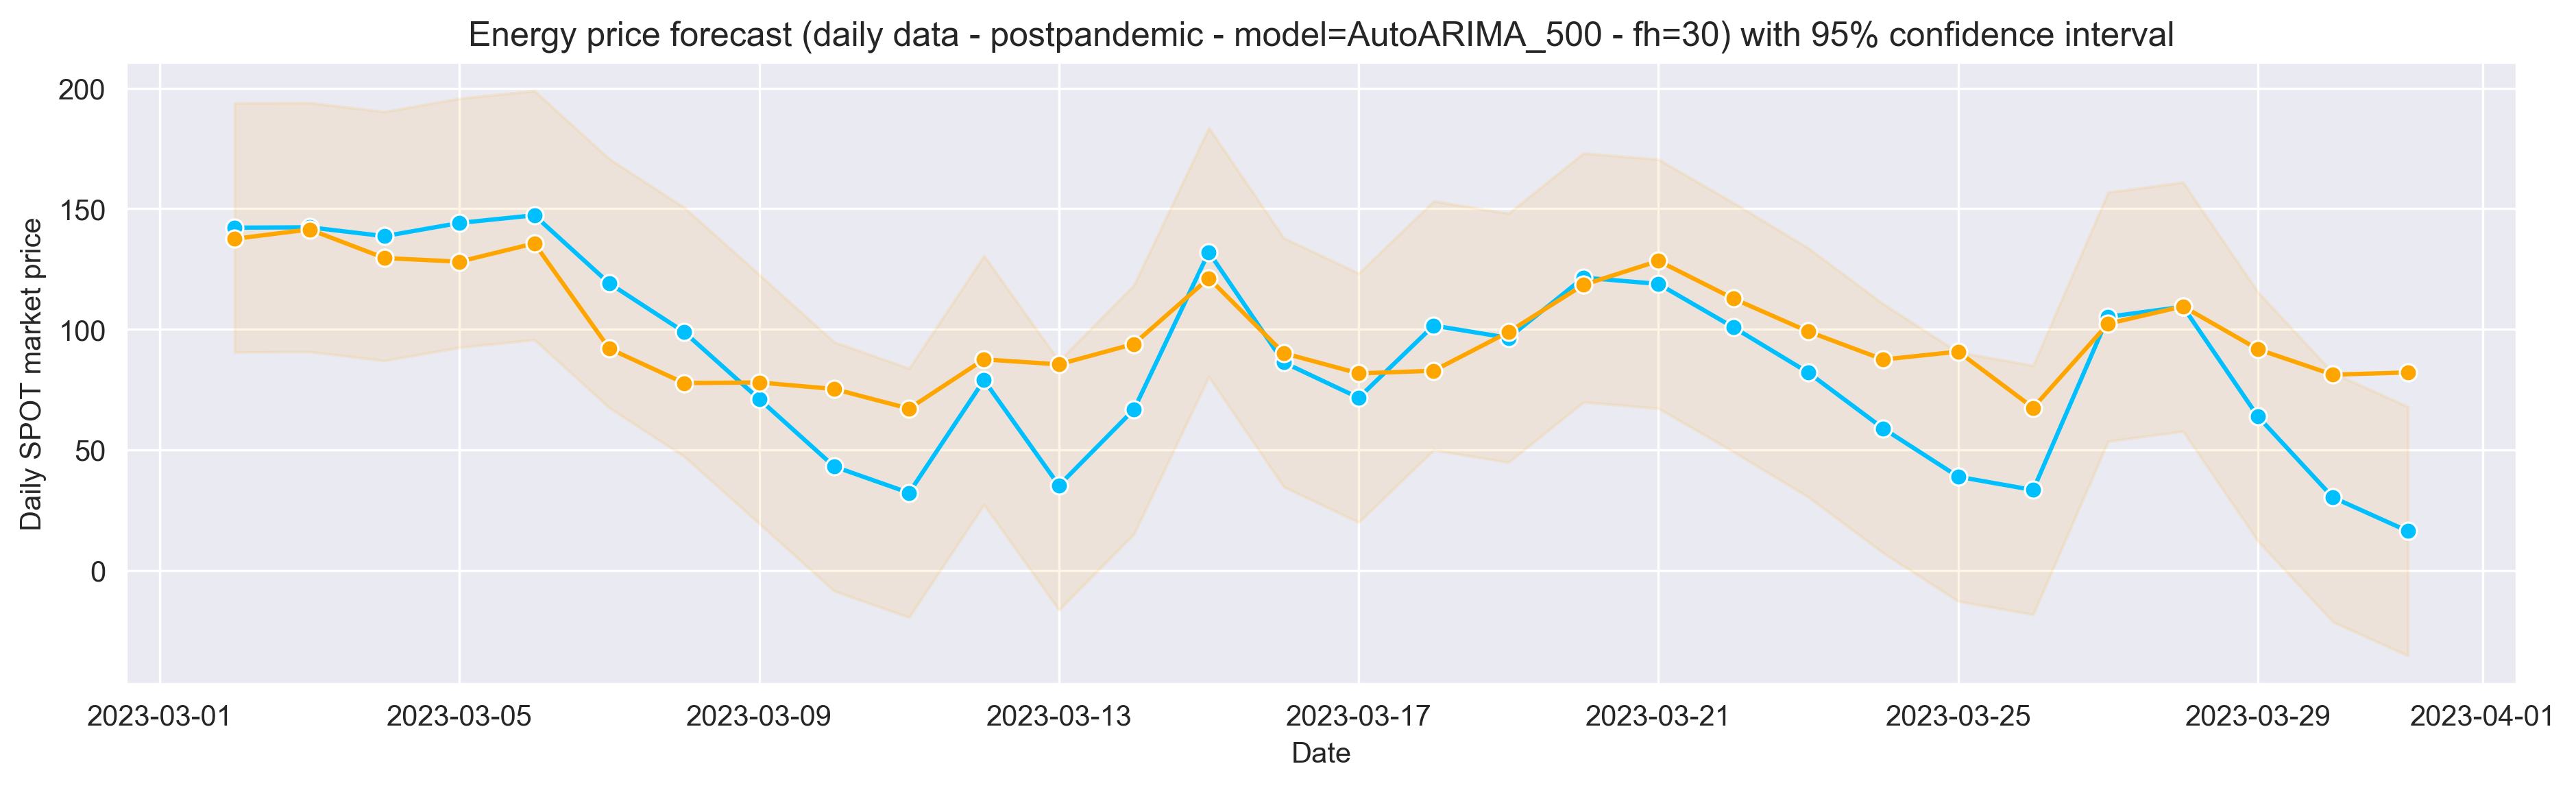
\includegraphics[scale=0.4]{images/analysis/forecast-arima-daily-post}}
\end{figure}

Looking at SHAP values we see similar tendencies to what seen in the pre-pandemic situation. Clean energies tend to reduce price while commodity-based generation technologies increase it. Nevertheless, the impact on the model output in the post-war situation is generally higher because the SHAP values show also larger values.

\begin{figure}[H]
\centering
    \begin{subfigure}{.45\textwidth}
        \centering
        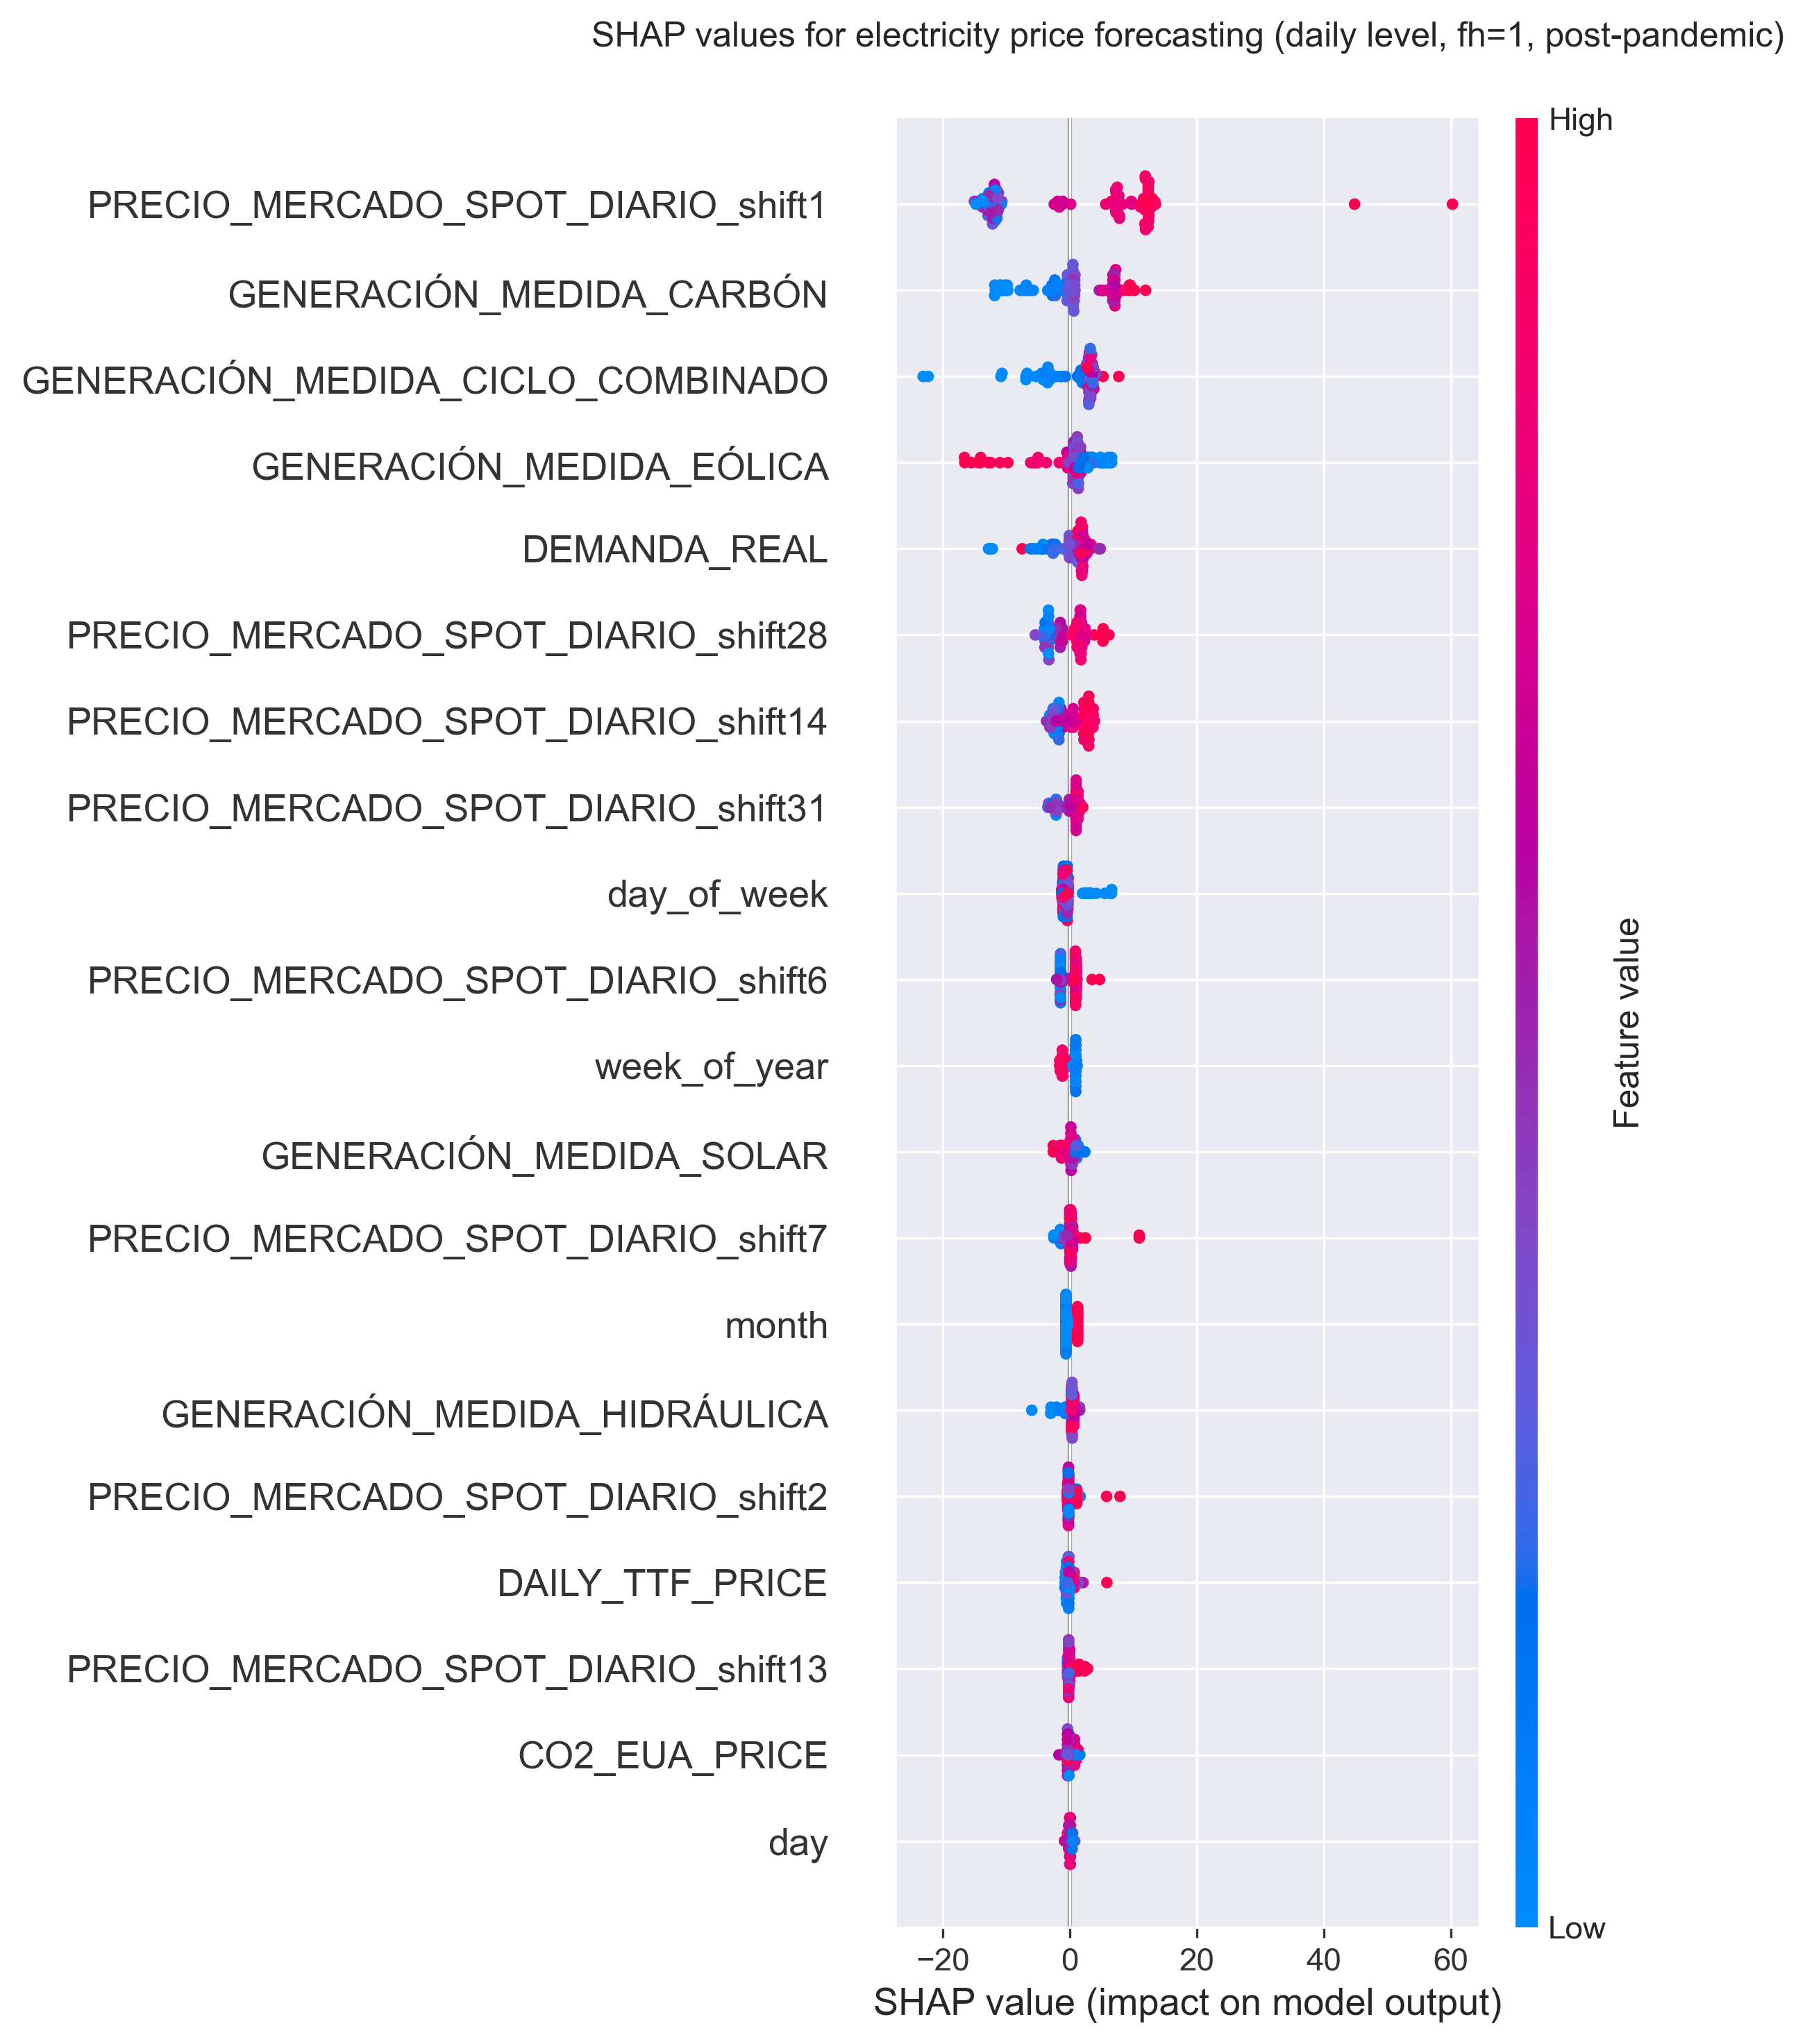
\includegraphics[width=1\linewidth]{images/analysis/shap-daily-post-1}
        \caption{fh=1}
    \end{subfigure}
    \begin{subfigure}{.45\textwidth}
        \centering
        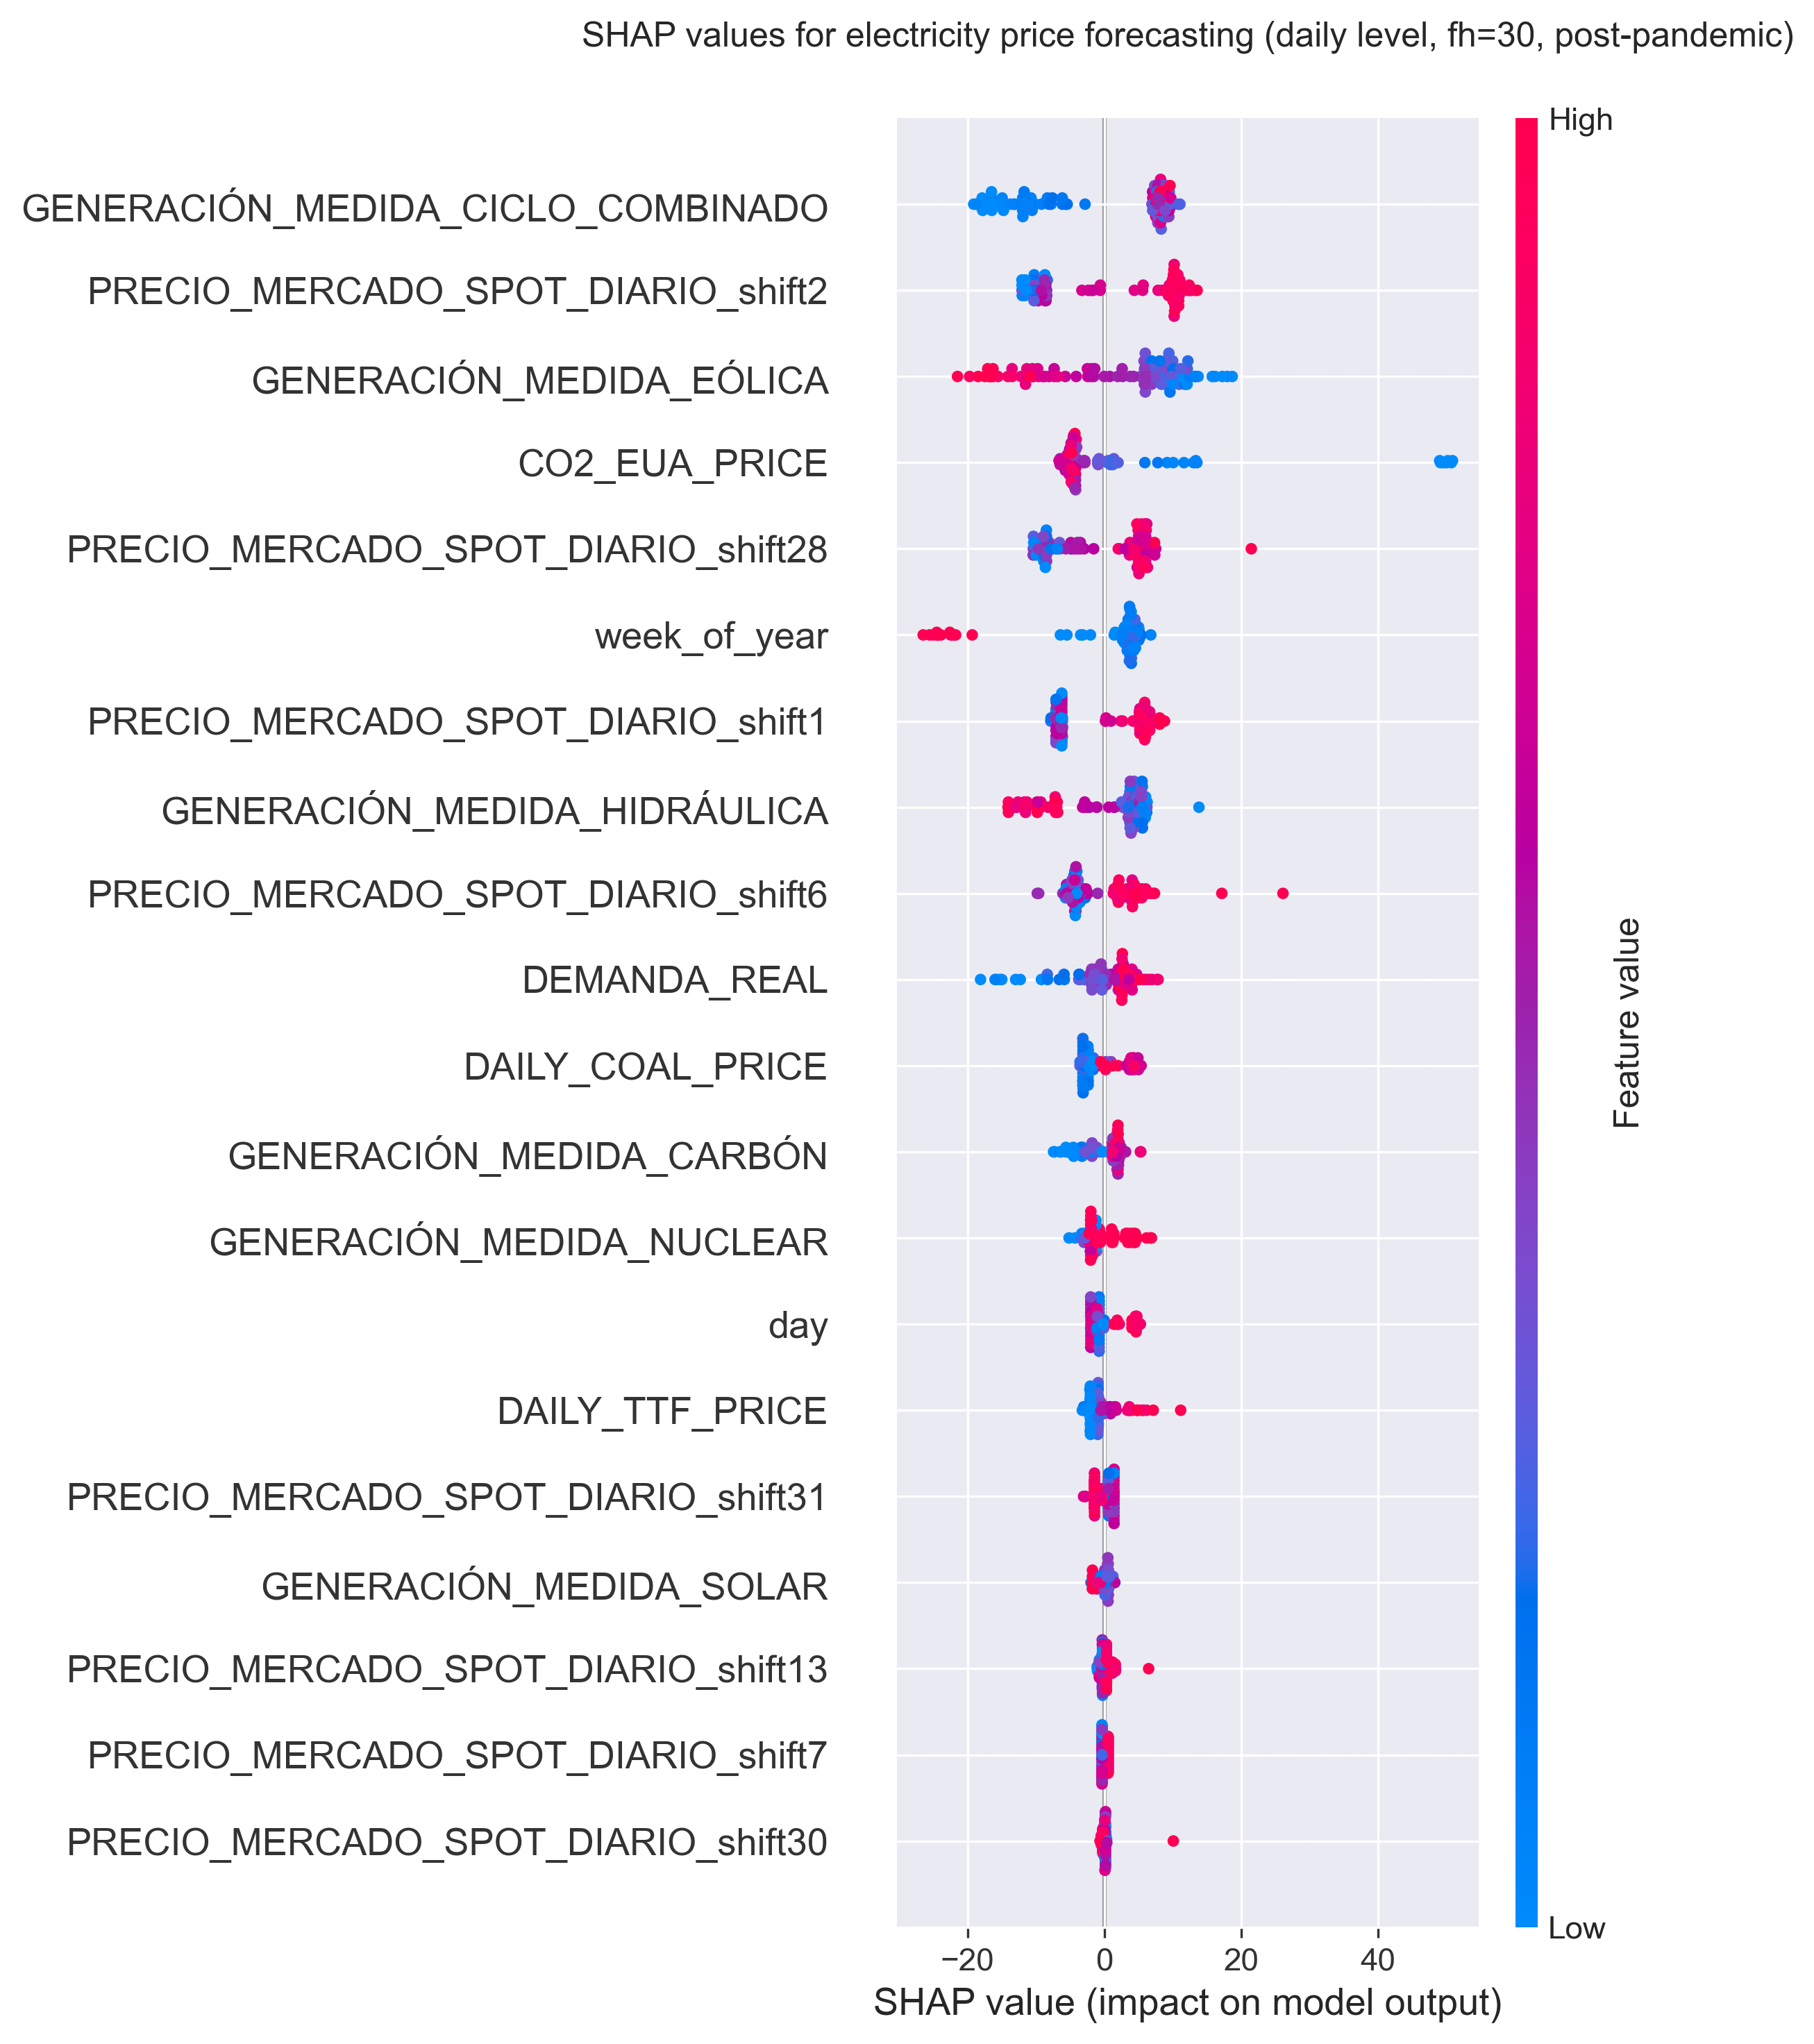
\includegraphics[width=1\linewidth]{images/analysis/shap-daily-post-30}
        \caption{fh=30}
    \end{subfigure}

    \caption{SHAP values for the daily post-war energy price forecasting.}
    \label{fig:shap-daily-post}
\end{figure}

\subsection{Result discussion}
TODO



\section{Monthly analysis}
In the monthly level the author won't compare pre-pandemic with post-war markets as there are no enough datapoints. He will perform the study over the complete series, with data from 2014-01 to 2023-03.

The same predictors as before are used, except those related with date, which change:
\begin{itemize}
    \item \textbf{Date predictors:} Month and year.
\end{itemize}

The best model now is the one based on Support Vector Machine

\begin{table}[H]
\centering
\begin{tabular}{l|l|l}
\hline
Model & MASE      & Fit time  \\ \hline
SVM   & 9.756828  & 0.120174  \\
DR    & 9.810081  & 0.079708  \\
RF    & 10.604719 & 16.363083 \\
kNN   & 10.676818 & 0.126496  \\
GBT   & 10.715059 & 4.840854  \\ \hline
\end{tabular}
\caption{}
\label{tab:cv-daily}
\end{table}

\begin{table}[]
\centering
\begin{tabular}{@{}l|l|l@{}}
\toprule
Model         & MASE     & Fit time   \\ \midrule
AutoARIMA\_48 & 1.776982 & 114.29715  \\
AutoARIMA\_36 & 2.023715 & 124.680216 \\
AutoARIMA\_24 & 2.046998 & 68.49768   \\
AutoARIMA\_72 & 2.445332 & 67.781334  \\ \bottomrule
\end{tabular}
\caption{}
\label{tab:arima-monthly}
\end{table}

\begin{figure}[H]
\centering
    \caption{Final forecasting of monthly energy price.}
    \label{fig:forecast-arima-monthly}
    \fbox{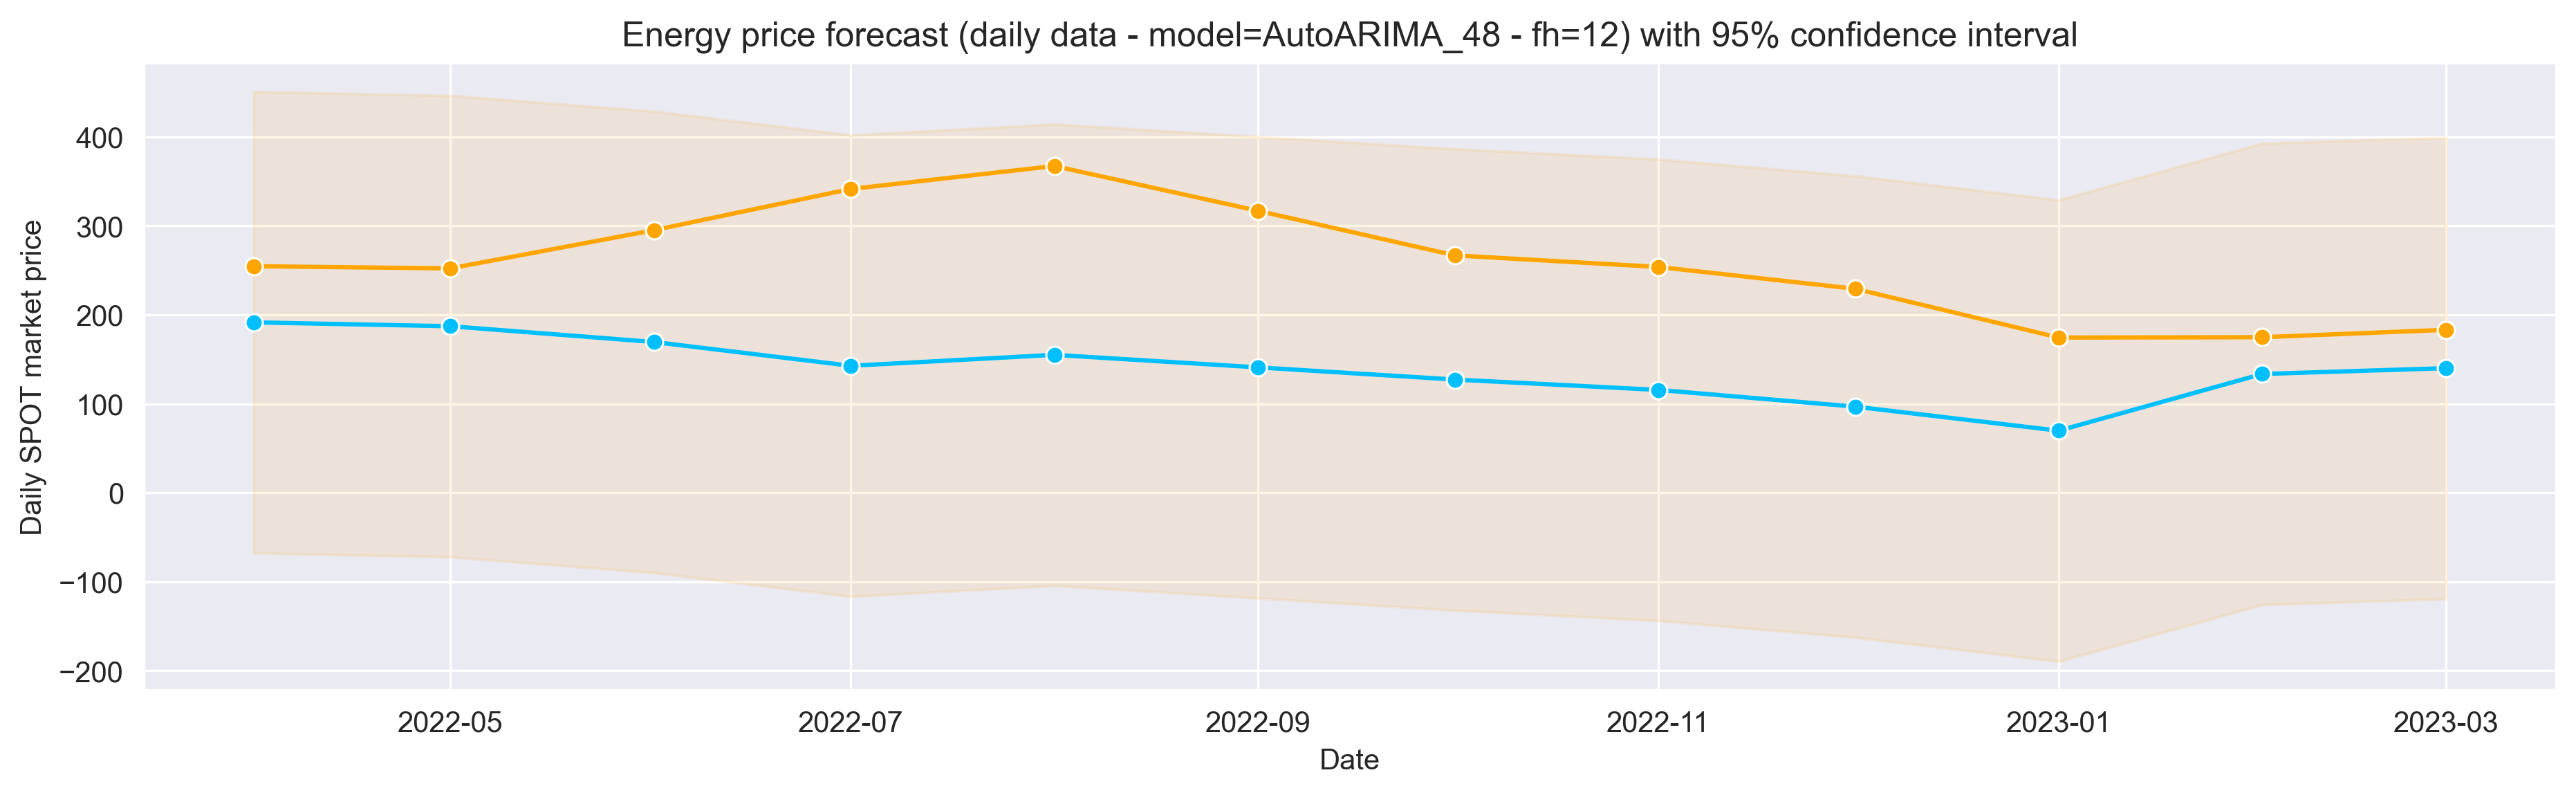
\includegraphics[scale=0.4]{images/analysis/forecast-arima-monthly}}
\end{figure}

\begin{figure}[H]
\centering
    \begin{subfigure}{.45\textwidth}
        \centering
        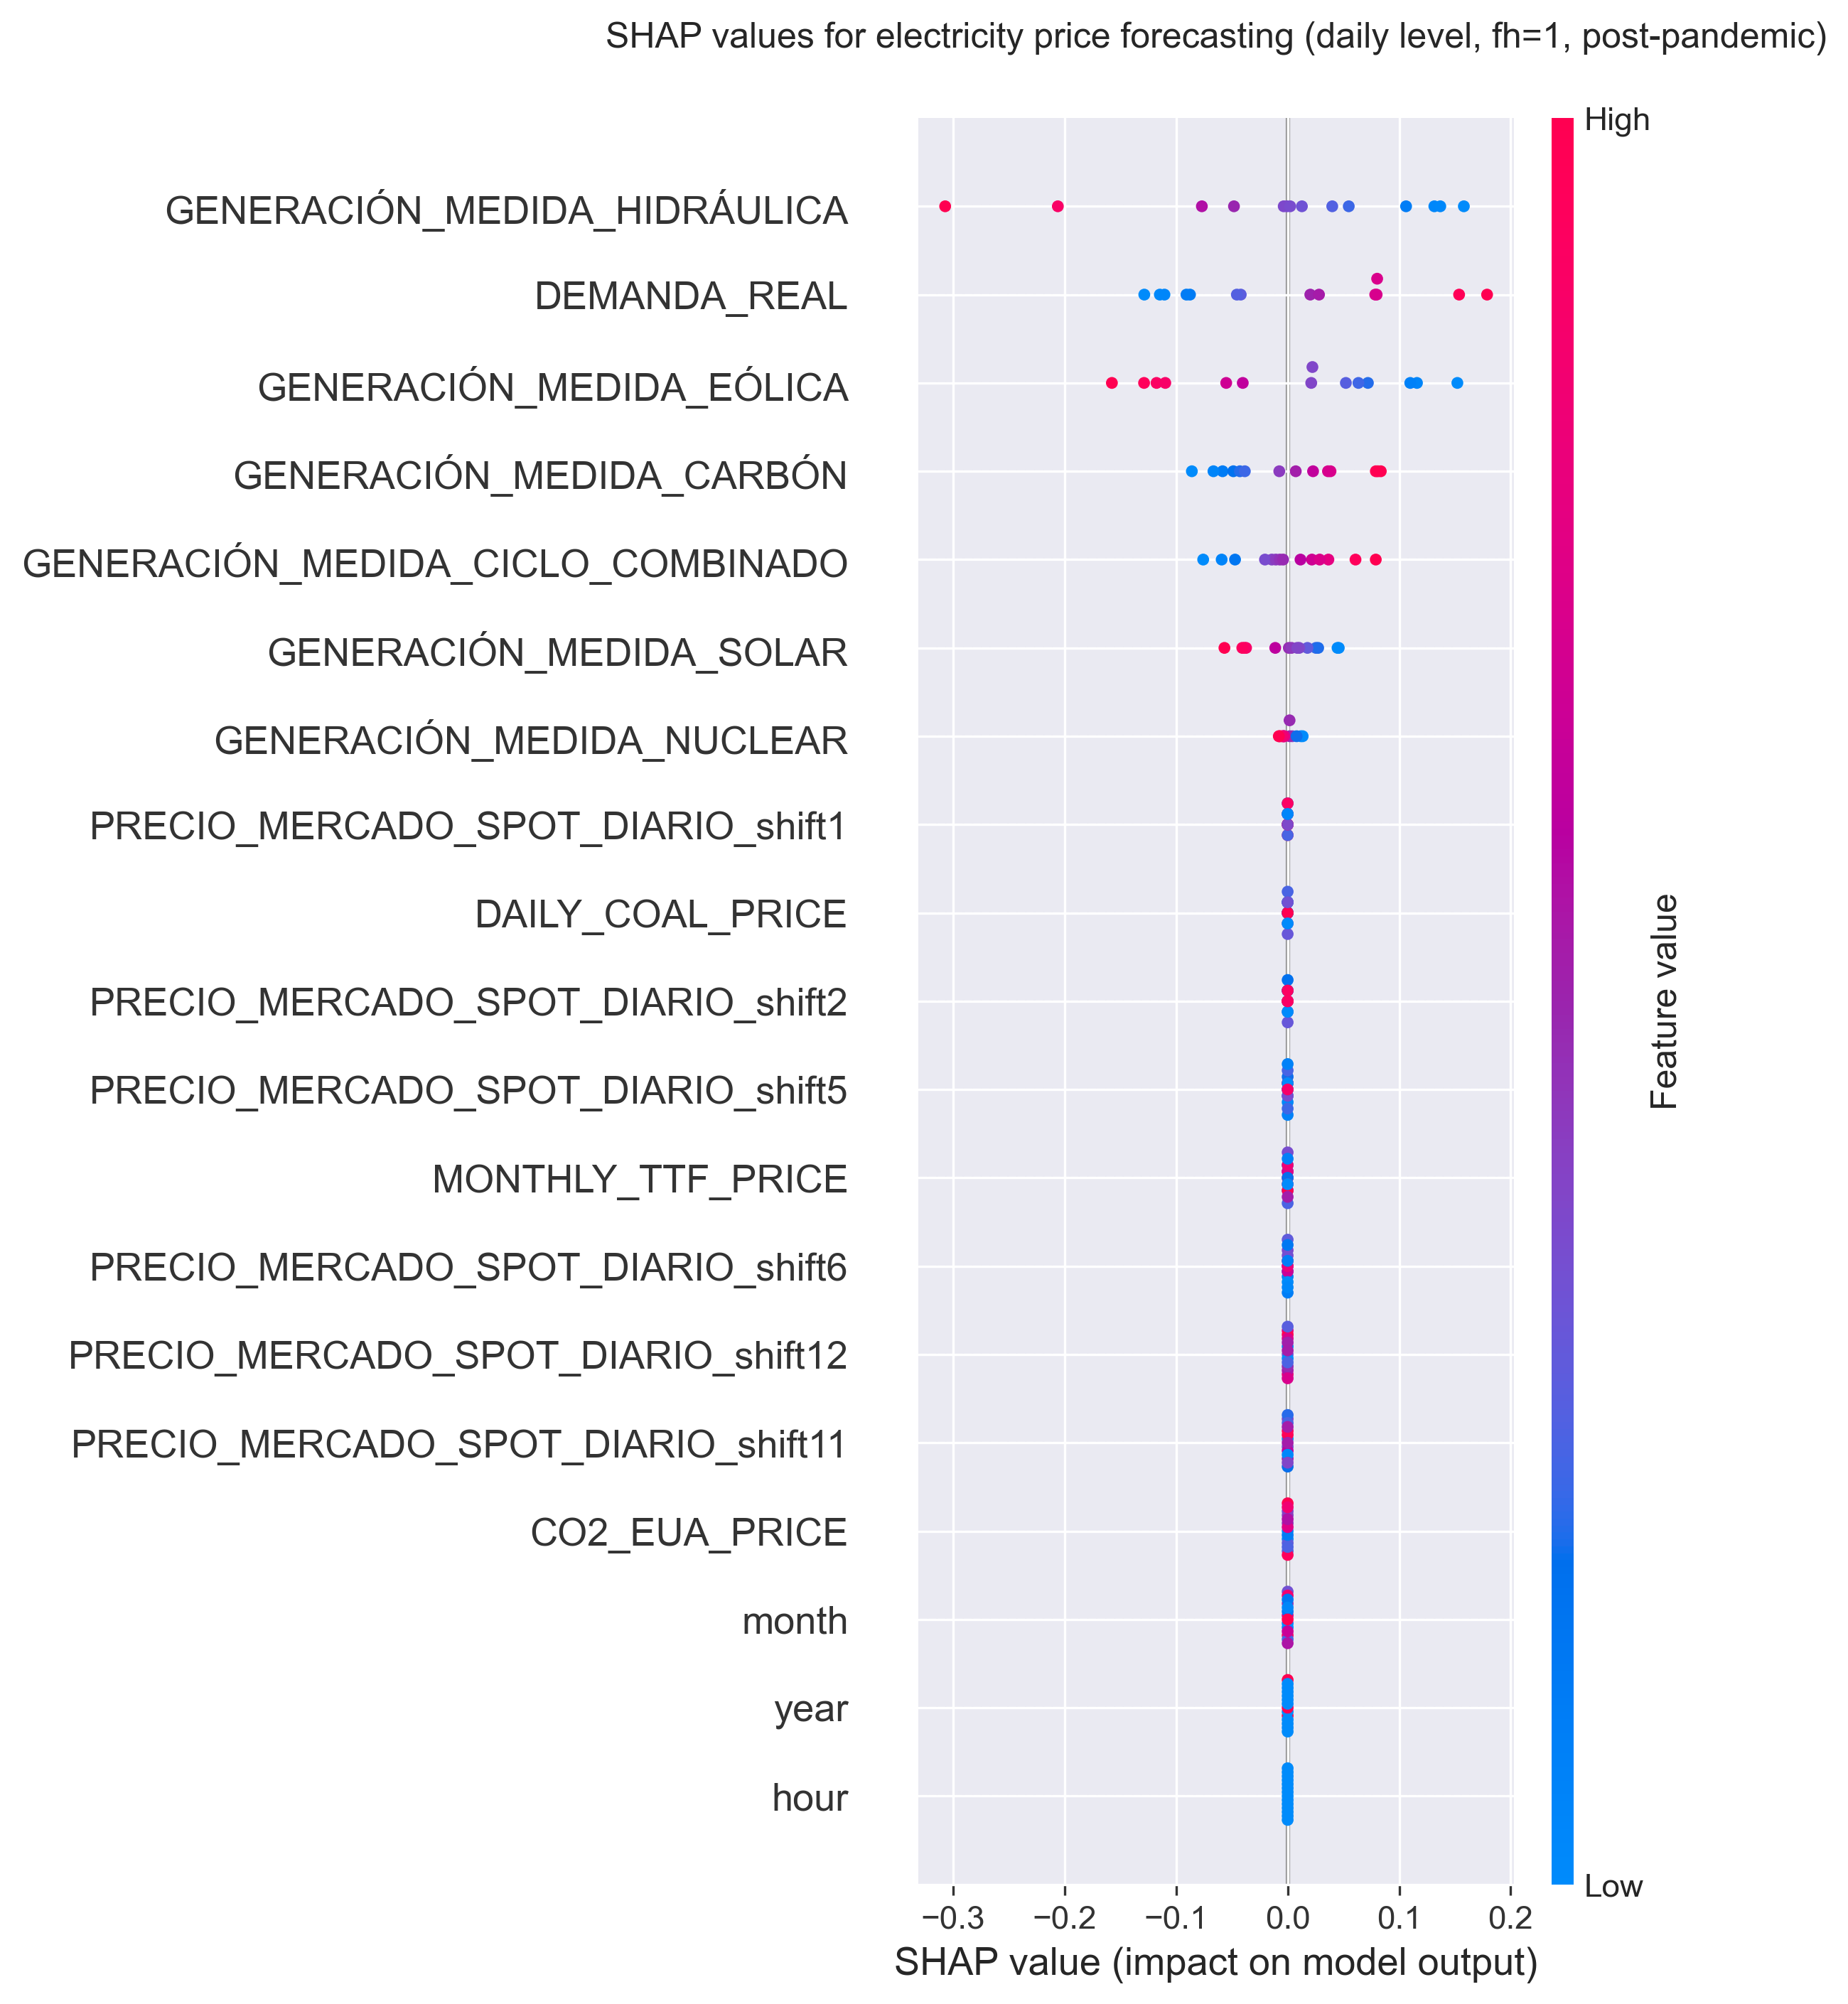
\includegraphics[width=1\linewidth]{images/analysis/shap-monthly-1}
        \caption{fh=1}
    \end{subfigure}
    \begin{subfigure}{.45\textwidth}
        \centering
        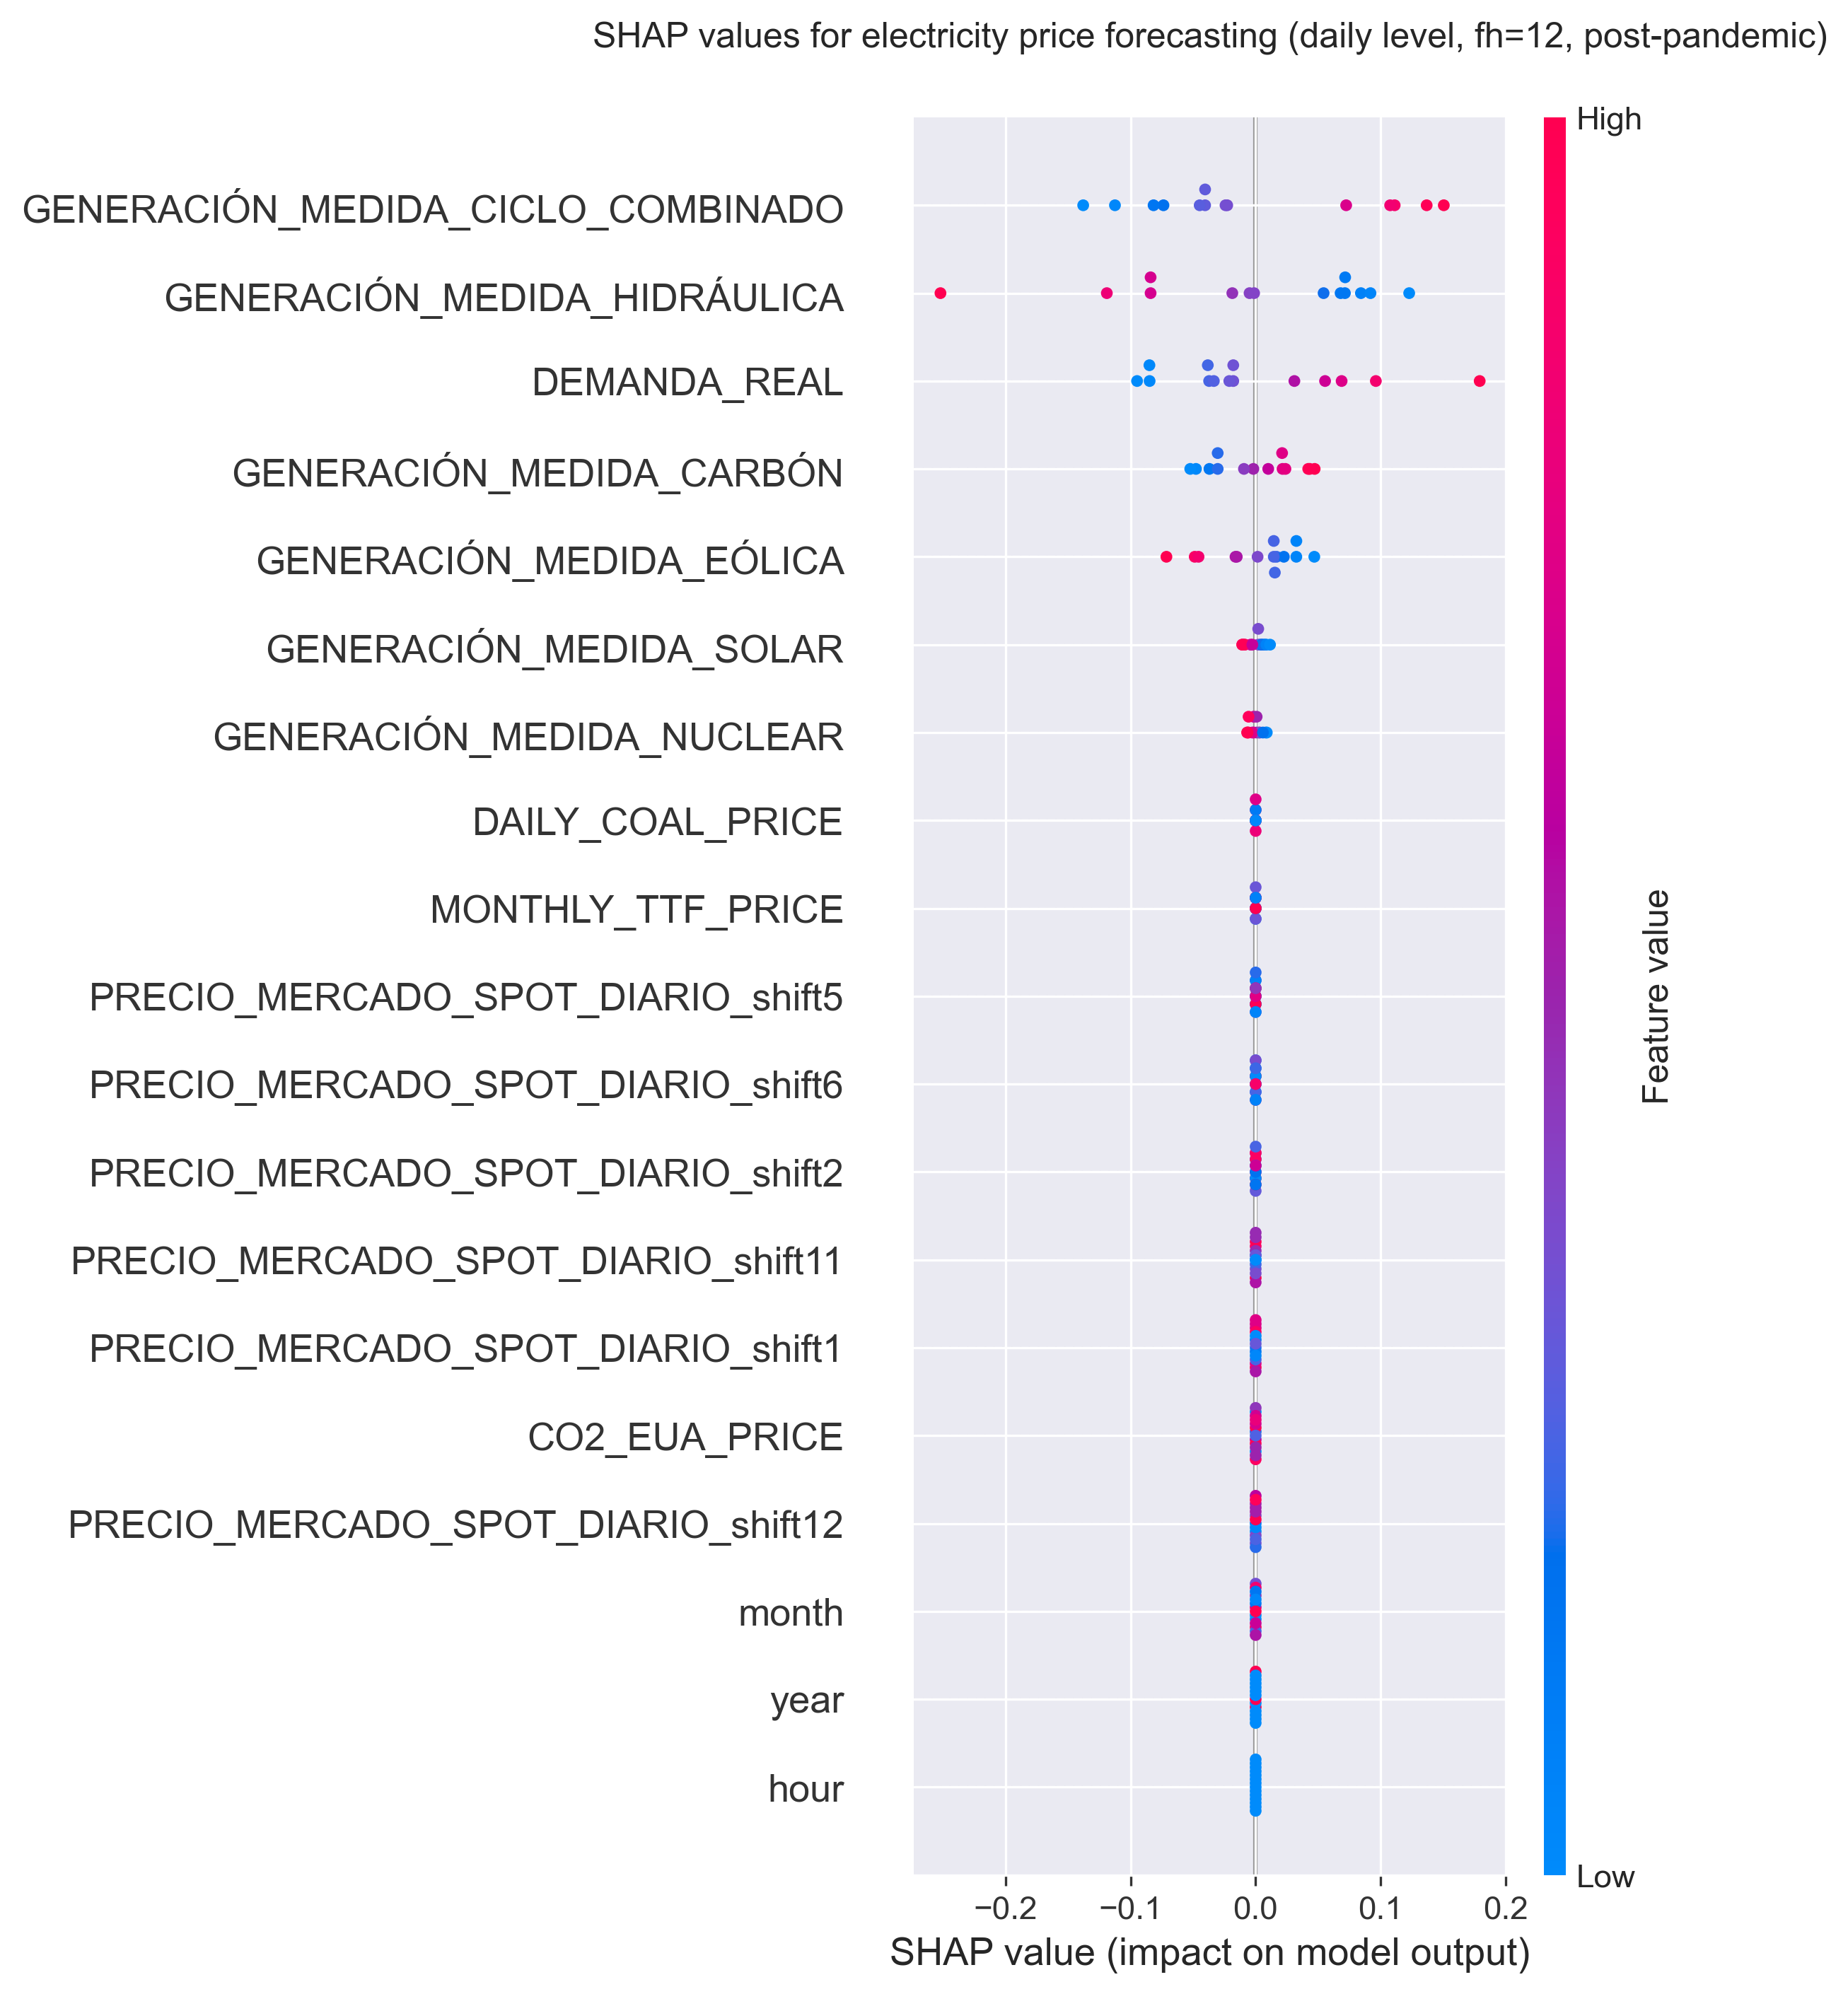
\includegraphics[width=1\linewidth]{images/analysis/shap-monthly-12}
        \caption{fh=12}
    \end{subfigure}

    \caption{SHAP values for the monthly energy price forecasting.}
    \label{fig:shap-monthly}
\end{figure}



\section{Yearly analysis}